
\documentclass[spanish,openright]{book}

%%%%%%%%%%%%%%%%%%%%%%%%%%%%%%%%%%%%%%%%%%%%%%%%%%%%%%%%%%%%%%%%%%%%%%%%%%%
% Comienzo del Preamble y seccion de configuracion
%

%% FIXING PROBLEM WITH ALL PAGES PRINTED IN COLOR \documentclass[RGB,rgb,svgnames,spanish,openright]{book}
%\documentclass[spanish,openright]{book}
% \documentclass[english,openright]{book}
% \documentclass[11pt,english,twoside,openright]{book}

% \usepackage[a4,cam,center]{crop}
% \crop[font=\upshape\mdseries\small\textsf]

\synctex=1

% ifthen to allow using language dependent settings
\usepackage{ifthen}

%% JMG: FIXING PROBLEM WITH ALL PAGES PRINTED IN COLOR
% This should not be touched, as it should work as it is know.
\newcommand{\colorspaceused}{rgb}

%The next section seems to be useless, but it's still pending to try further
\ifthenelse{\equal{\colorspaceused}{rgb}}
{
  \PassOptionsToPackage{rgb}{xcolor}% NB: put this *before* \usepackage{pst-all}
}
{
  \PassOptionsToPackage{cmyk}{xcolor}% NB: put this *before* \usepackage{pst-all}
}

%\usepackage[latin1]{inputenc} % Para poder escribir con acentos y ñ. en
                              % latin1
\usepackage[utf8]{inputenc} % Para poder escribir con acentos y ñ. en utf8
\usepackage[T1]{fontenc}      % Para que haga bien la ``hyphenation''. No
                              % usar si no es necesario, porque ralentiza muchisimo la compilación.
\usepackage{ae}               % Para que todas las fuentes sean Type1, y ninguna Type3.
\usepackage{lmodern}          % This generates a pdf with searchable
                              % accented characters!!!!!!!!!!!!!!!!!!!!!!!!!!!!!!!!!!!!!!!


\usepackage{wrapfig}
\usepackage{lipsum}

% Use this if you want to include pdf files in the final document
\usepackage[final]{pdfpages}

% Use this if you want to delete headers and footers in empty pages
\usepackage{emptypage}

% \usepackage[nottoc]{tocbibind}
\usepackage{tocbibind}

\usepackage{listings}
\usepackage{longtable}
\usepackage{afterpage}

\usepackage{xspace}
\usepackage{verbatim}
\usepackage{moreverb}
\usepackage{multicol}
\usepackage{amsmath}
\usepackage{eurosym}
%\usepackage{subfig} % subfigure is obsolete... 
\usepackage{multirow}
\usepackage{fancyhdr}
\usepackage{makeidx}
\usepackage{rotating}
\usepackage{supertabular}
\usepackage{hhline}
\usepackage{array}
\usepackage[noadjust]{cite}     

\usepackage[center]{caption}
\usepackage{subcaption}

%% FIXING PROBLEM WITH ALL PAGES PRINTED IN COLOR
\usepackage{xcolor}
% \usepackage[RGB,rgb]{xcolor}
% \usepackage{color}
% Pantone 160
% \definecolor{headingPortadaTFM}{RGB}{158,84,10}
% Pantone 160C (this is supposed to be the correct one, but it looks horrible in screen)
% \definecolor{headingPortadaTFM}{RGB}{161,86,28}
% Gold in RGB
% \definecolor{textoHeadingPortadaTFM}{RGB}{215,215,0}
% Captured colors in screen (this looks pst on screen)

% \ifthenelse{\equal{\colorspaceused}{rgb}}
% {
%   \definecolor{headingPortadaTFM}{RGB}{152,118,52}
%   \definecolor{textoHeadingPortadaTFM}{RGB}{208,205,102}
% }
% {
%   % These definitions are for cmyk colorspace
%   \definecolor{headingPortadaTFM}{cmyk}{0.0254,0,0.559,0.537}
%   \definecolor{textoHeadingPortadaTFM}{cmyk}{0,0.0144,0.51,0.184}
% }

\definecolor{pantone293}{RGB}{35,91,168}

\definecolor{headingPortadaTFG}{RGB}{152,118,52}
\definecolor{headingPortadaTFM}{RGB}{0,90,170}
\definecolor{textoHeadingPortadaTFM}{RGB}{208,205,102}
\definecolor{textoHeadingPortadaTFG}{RGB}{208,205,102}

\definecolor{gray97}{gray}{.97}
\definecolor{gray75}{gray}{.75}
\definecolor{gray45}{gray}{.45}




% To draw rectagles in tfm cover
\usepackage{tikz}

\usepackage{Sweave}


% \usepackage[authoryear]{natbib}
% \makeatletter
% \let\NAT@parse\undefined
% \makeatother
% \usepackage{natbib}

\usepackage{geometry}
\geometry{verbose,a4paper,tmargin=2.5cm,bmargin=2.5cm,lmargin=2.5cm,rmargin=2.5cm}
% \geometry{paperwidth=210mm,paperheight=297mm}

%\usepackage[hang, flushmargin]{footmisc}   

\usepackage[
%% ps2pdf,                %%% hyper-references for ps2pdf
bookmarks=true,%                   %%% generate bookmarks ...
bookmarksnumbered=true,            %%% ... with numbers
hypertexnames=false,               %%% needed for correct links to
%%% figures!!!
% hypertexnames=true,               %%% needed for correct links on pagebackrefs!!!
breaklinks=true,                   %%% breaks lines, but links are very small
% pagebackref=true,
% linktocpage=true,                 %%% enlace en el numero de página.
linktoc=all,
colorlinks=true,
linkcolor=blue,    
citecolor=green,
urlcolor=blue,                     %%% texto  con color (further
%%% modified in myconfig.tex)
% linkbordercolor={0 0 1},           %%% blue frames around links
pdfborder={0 0 112.0},              %%% border-width of frames 
hyperfootnotes=false,
]{hyperref}                        %%% will be multiplied with 0.009 by ps2pdf
%\usepackage[all]{hypcap}

% Para numerar las \subsubsection
\setcounter{secnumdepth}{5}
% para hacer que las \subsubsection aparezcan en el indice
\setcounter{tocdepth}{5}
% \setcounter{lofdepth}{2}
\setcounter{table}{1}
\setcounter{figure}{1}
\setcounter{secnumdepth}{4}


\setlength{\parskip}{1ex plus 0.5ex minus 0.2ex}


\usepackage{multirow}

\usepackage{setspace}
% \renewcommand{\baselinestretch}{10}
\newcommand{\mycaptiontable}[1]{
  \begin{spacing}{0.6}
    % \vspace{0.5cm}
    \begin{quote}
      % \begin{center}
      {{Table} \thechapter.\arabic{table}: #1}
      % \end{center}
    \end{quote}
    % \vspace{1cm}
  \end{spacing}
  \stepcounter{table}
}

\newcommand{\mycaptionfigure}[1]{
  % \vspace{0.5cm}
  \begin{spacing}{0.6}
    \begin{quote}
      % \begin{center}
      {{Figure} \thechapter.\arabic{figure}: #1}
      % \end{center}
    \end{quote}
    % \vspace{1cm}
  \end{spacing}
  \stepcounter{figure}
}

\usepackage{amsmath}

\usepackage{courier}

% ***************************************************************************
% ***************************************************************************
% ***************************************************************************
\usepackage{multirow}
\usepackage{rotating}
\usepackage{setspace, amssymb, amsmath, epsfig, multirow, colortbl, tabularx}%
% For acronym package:
% If footnote is specified, text will be included in a footnote
% If printonlyused is specified, only used acronyms will be included
% I use the acronym sty under the sty directory as I needed the newest version
% \usepackage[footnote,printonlyused,withpage]{acronym} 
% \usepackage[printonlyused]{sty/acronym}

% glossaries is better than the acronym package 
\usepackage[acronym,shortcuts,nomain,hyperfirst=false]{glossaries}
% If you want to PERMANENTLY DISABLE HYPERLINKS, uncomment the following
% line
% \glsdisablehyper
% In future versiones (not as for ubuntu 12.04) You can also selectively
% disable hyperlinks for given glossaries, using:
% \usepackage[acronym,shortcuts,nomain,nohypertypes={acronyms,symbols}]{glossaries}
% Or (for newwer versions also), you can even use
% \GlsDeclareNoHyperList{acronyms,symbols}
% You can also disable hyperlinks in the acronym use, like in \ac*{symbol}


\newcommand{\clearemptydoublepage}{\newpage{\pagestyle{empty}\cleardoublepage}}

\pagestyle{fancy}

\providecommand\phantomsection{}
\onehalfspacing
\sloppy  %better line breaks

\renewcommand{\chaptermark}[1]{\markboth{\chaptername\ \thechapter.\ #1}{}}
\renewcommand{\sectionmark}[1]{\markright{\thesection\ #1}{}}

%%%%%%%%%%%%%%%%%%%%%%%%%%%%%%%%%%%%%%%%%%%%%%%%%%%%%%%%%%%%%%%%%%%%%%%%%%% 
% BEGIN Fancy headers stuff
\fancyhf{}

\fancyhead[LE,RO]{\bfseries\thepage}
\fancyhead[LO]{\bfseries\rightmark}
\fancyhead[RE]{\bfseries\leftmark}

\makeatletter
\renewcommand{\chaptermark}[1]{\markboth{\@chapapp \ \thechapter . \ #1}{}}
\renewcommand{\sectionmark}[1]{\markright{\thesection \ \ #1}}
\makeatother

\renewcommand{\headrulewidth}{0.5pt}
\renewcommand{\footrulewidth}{0pt}
\addtolength{\headheight}{3.5pt}
\fancypagestyle{plain}{\fancyhead{}\renewcommand{\headrulewidth}{0pt}}
\fancypagestyle{myplain}
{
  \fancyhf{}
  \renewcommand\headrulewidth{0pt}
  \renewcommand\footrulewidth{0pt}
  \fancyfoot[C]{\thepage}
}
% END Fancy headers stuff
%%%%%%%%%%%%%%%%%%%%%%%%%%%%%%%%%%%%%%%%%%%%%%%%%%%%%%%%%%%%%%%%%%%%%%%%%%% 

%%%%%%%%%%%%%%%%%%%%%%%%%%%%%%%%%%%%%%%%%%%%%%%%%%%%%%%%%%%%%%%%%%%%%%%%%%% 
% BEGIN Set nice chapter titles

% BEGIN Example 0 from http://texblog.org/2012/07/03/fancy-latex-chapter-styles/
% \usepackage[explicit]{titlesec}
% \usepackage{blindtext}
% \definecolor{gray75}{gray}{0.75}
% \newcommand{\hsp}{\hspace{20pt}}
% \titleformat{\chapter}[hang]{\Huge\bfseries}{\chaptername~\thechapter\hsp\textcolor{gray75}{|}\hsp}{0pt}{\Huge\bfseries}
% END Example 0 from http://texblog.org/2012/07/03/fancy-latex-chapter-styles/

% BEGIN Example 1 from http://texblog.org/2012/07/03/fancy-latex-chapter-styles/
% \usepackage{titlesec}
% \usepackage{blindtext}
% \definecolor{gray75}{gray}{0.75}
% \newcommand{\hsp}{\hspace{20pt}}
% \titleformat{\chapter}[hang]{\Huge\bfseries}{\chaptername~\thechapter\hsp\textcolor{gray75}{|}\hsp}{0pt}{\Huge\bfseries}
% END Example 1 from http://texblog.org/2012/07/03/fancy-latex-chapter-styles/

% BEGIN Example 2 from http://texblog.org/2012/07/03/fancy-latex-chapter-styles/
% Options: Sonny, Lenny, Glenn, Conny, Rejne, Bjarne, Bjornstrup
% \usepackage[Sonny]{fncychap}
% \usepackage[Lenny]{fncychap} % ugly
% \usepackage[Glenn]{fncychap}
% \usepackage[Conny]{fncychap} % ugly
% \usepackage[Rejne]{fncychap}
% \usepackage[Bjarne]{fncychap} % Doesn't work in Spanish
% \usepackage[Bjornstrup]{fncychap}
% END   Example 2 from http://texblog.org/2012/07/03/fancy-latex-chapter-styles/

% BEGIN Example 3 from http://texblog.org/2012/07/03/fancy-latex-chapter-styles/
% This is a nice colored example
% \usepackage{kpfonts}
% \usepackage[explicit]{titlesec}
% \newcommand*\chapterlabel{}
% \titleformat{\chapter}
% {\gdef\chapterlabel{}
% \normalfont\sffamily\Huge\bfseries\scshape}
% {\gdef\chapterlabel{\thechapter\ }}{0pt}
% {\begin{tikzpicture}[remember picture,overlay]
%   \node[yshift=-3cm] at (current page.north west)
%   {\begin{tikzpicture}[remember picture, overlay]
%     \draw[fill=LightSkyBlue] (0,0) rectangle
%     (\paperwidth,3cm);
%     \node[anchor=east,xshift=.9\paperwidth,rectangle,
%     rounded corners=20pt,inner sep=11pt,
%     fill=MidnightBlue]
%     {\color{white}\chapterlabel#1};
%   \end{tikzpicture}
% };
% \end{tikzpicture}
% }
%   \titlespacing*{\chapter}{0pt}{50pt}{-60pt}
%   END   Example 3 from http://texblog.org/2012/07/03/fancy-latex-chapter-styles/

%   BEGIN Example 4 from http://texblog.org/2012/07/03/fancy-latex-chapter-styles/
%   END   Example 4 from http://texblog.org/2012/07/03/fancy-latex-chapter-styles/


%   END Set nice chapter titles
%%%%%%%%%%%%%%%%%%%%%%%%%%%%%%%%%%%%%%%%%%%%%%%%%%%%%%%%%%%%%%%%%%%%%%%%%%%   

%%%%%%%%%%%%%%%%%%%%%%%%%%%%%%%%%%%%%%%%%%%%%%%%%%%%%%%%%%%%%%%%%%%%%%%%%%%   
%   This is to set background images (in our case to set background image
%   in TFMs front and back pages)
%   If you want to set this background, use \BgThispage in the
%   corresponding pages
%\usepackage[pages=some]{sty/background}
\usepackage[pages=some]{background}

\ifthenelse{\equal{\colorspaceused}{rgb}}
{
  \backgroundsetup{ scale=1, angle=0, opacity=.1, color=pink,
    contents={
\includegraphics[width=.7\paperwidth]{logos/logoEPS-UAH.jpg}}, vshift=-50pt,  hshift=0pt }
}
{
  \backgroundsetup{ scale=1, angle=0, opacity=.1, color=pink,
    contents={
\includegraphics[width=.7\paperwidth]{logos/logoEPS-UAH-cmyk.jpg}}, vshift=-50pt,  hshift=0pt }
}


% This is to allow do a clearpage and let the next one to be placed in
% even pages (to set a backpage for example)
\makeatletter
\newcommand*{\cleartoleftpage}{%
  \clearpage
  \if@twoside
  \ifodd\c@page
  \hbox{}\newpage
  \if@twocolumn
  \hbox{}\newpage
  \fi
  \fi
  \fi
}
\makeatother

% Let's define some styles for source code listings:
% 
% minimizar fragmentado de listados (from
% http://www.rafalinux.com/?p=599), pero no me funciona:
% \lstnewenvironment{codelisting}[1][]
% {\lstset{#1}\pagebreak[0]}{\pagebreak[0]}
% 
% This was using the float package
\usepackage{float}
\floatstyle{plaintop} % optionally change the style of the new float
\newfloat{codefloat}{H}{cod}[chapter]

\lstdefinestyle{console}
{
  basicstyle=\scriptsize\bf\ttfamily,
  backgroundcolor=\color{gray75},
}

\lstdefinestyle{Cbluebox}
{
  language=C,
  frame=shadowbox, 
  rulesepcolor=\color{blue}
}

\lstdefinestyle{Cnice}
{
  language=C,
  frame=Ltb,
  framerule=0pt,
  tabsize=2,
  aboveskip=0.5cm,
  framextopmargin=3pt,
  framexbottommargin=3pt,
  framexleftmargin=0.4cm,
  framesep=0pt,
  rulesep=.4pt,
  backgroundcolor=\color{gray97},
  rulesepcolor=\color{black},
  % 
  stringstyle=\ttfamily,
  showstringspaces = false,
  % basicstyle=\small\ttfamily,
  basicstyle=\footnotesize\ttfamily,
  commentstyle=\color{gray45},
  keywordstyle=\bfseries,
  % 
  numbers=left,
  numbersep=15pt,
  numberstyle=\tiny,
  numberfirstline = false,
  breaklines=true,
}	

\lstdefinestyle{CppExample}
{
  language=C++,
  frame=trbl,
  tabsize=2,
  commentstyle=\textit,
  stringstyle=\ttfamily, 
  basicstyle=\small,
}	

% This one from http://en.wikibooks.org/wiki/LaTeX/Source_Code_Listings
\lstdefinestyle{Ccolor}
{
  belowcaptionskip=1\baselineskip,
  breaklines=true,
  frame=L,
  xleftmargin=\parindent,
  language=C,
  showstringspaces=false,
  basicstyle=\footnotesize\ttfamily,
  keywordstyle=\bfseries\color{green!40!black},
  commentstyle=\itshape\color{purple!40!black},
  identifierstyle=\color{blue},
  stringstyle=\color{orange},
}

% From http://tex.stackexchange.com/questions/46953/unix-command-highlighting-latex
\lstdefinestyle{BashInputStyle}{
  language=bash,
  basicstyle=\small\sffamily,
  numbers=left,
  numberstyle=\tiny,
  numbersep=3pt,
  frame=tb, 
  showspaces=false, 
  showtabs=false,
  showstringspaces=false,
  columns=fullflexible,
  backgroundcolor=\color{gray97},
  % backgroundcolor=\color{yellow!20},
  linewidth=0.9\linewidth,
  xleftmargin=0.05\linewidth
}


% To set side-captions in figures
\usepackage{sidecap}

%%%%%%%%%%%%%%%%%%%%%%%%%%%%%%%%%%%%%%%%%%%%%%%%%%%%%%%%%%%%%%%%%%%%%%%%%%% 
% This comes from TeXiS, thanks to its authors, available at
% http://gaia.fdi.ucm.es/projects/texis 
\def\texis{\TeX \raise.15em\hbox{\textsc{i}}S}
%%%%%%%%%%%%%%%%%%%%%%%%%%%%%%%%%%%%%%%%%%%%%%%%%%%%%%%%%%%%%%%%%%%%%% 
% Comando:
% 
% \begin{FraseCelebre}
%   \begin{Frase}
%     Y así, del mucho leer y del poco dormir...
%   \end{Frase}
%   \begin{Fuente}
%     Don Quijote de la Mancha
%     
%     Miguel de Cervantes
%   \end{Fuente}
%   \begin{FraseCelebre}
%     
%     Resultado:
%     
%     Añade la frase célebre del principio de un capítulo.
%%%%%%%%%%%%%%%%%%%%%%%%%%%%%%%%%%%%%%%%%%%%%%%%%%%%%%%%%%%%%%%%%%%%%%     
\newenvironment{FraseCelebre}% Definición del entorno de FraseCelebre
{\begin{list}{}{%
      \setlength{\leftmargin}{0.5\textwidth}% Desplazamos el inicio de
      % los párrafos a la derecha la mitad
      % de la anchura de la línea de texto.
      % Puede que quieras cambiar esto
      % por otra cantidad como '5cm'.
      \setlength{\parsep}{0cm}% La separación entre párrafos de la
      % frase o de la fuente es normal, sin
      % espacio extra.
      \addtolength{\topsep}{0.5cm}% Aumentamos un poco la separación
      % entre la parte de la fase célebre
      % y los párrafos de alrededor
    }
  }
  {\unskip \end{list}}

\newenvironment{Frase}%
{\item \begin{flushright}\small\em}%
  {\end{flushright}}

\newenvironment{Fuente}%
{\item \begin{flushright}\small}%
  {\end{flushright}}


% To put paragraphs at page bottom
\newenvironment{bottomparagraph}{\par\vspace*{\fill}}{\clearpage}
% \newenvironment{bottomparagraph}{\par\vspace*{\fill}}{\clearemptydoublepage}

% Add algorithms april 2014
\usepackage[vlined,algochapter]{algorithm2e}
% Make this compatible with older/newer versions of the package
\providecommand{\DontPrintSemicolon}{\dontprintsemicolon}
\providecommand{\SetAlgoLined}{\SetLine}



% Add support for fonts at arbitrary sizes september 2014, for TFG's cover
\usepackage{fix-cm}

\usepackage{graphicx}                                                                      

% This is to avoid producing an hyperlink for starred documents. ONLY
% WORKS FOR THE ACRONYM PACKAGE, NOT USED HERE ANYMORE
% \makeatletter
% \AtBeginDocument{%
%   \renewcommand*\AC@hyperlink{%
%     \ifAC@starred
%       \expandafter\@secondoftwo
%     \else
%       \expandafter\hyperlink
%     \fi
%   }%
% }
% \makeatother

% This should be relative to the book.tex path, do not touch!!!!!!!!!!!
\newcommand{\myreferencespath}{}

%\providecommand{\DIFadd}[1]{{\protect\color{blue}#1}} %DIF PREAMBLE
%\providecommand{\DIFdel}[1]{{\protect\color{red}\protect\scriptsize{#1}}}

% As fancy underlining does not seem to compile with pdflatex, remove underline
%\providecommand{\DIFadd}[1]{{\protect\color{blue}{\protect\uwave{#1}}}}
\providecommand{\DIFadd}[1]{{\protect\color{blue}\textbf{#1}}}
\providecommand{\DIFdel}[1]{{\protect\color{red}\sout{#1}}}                     


%%%%%%%%%%%%%%%%%%%%%%%%%%%%%%%%%%%%%%%%%%%%%%%%%%%%%%%%%%%%%%%%%%%%%%%%%%%
% 
\usepackage{ifpdf}
\ifpdf
  \DeclareGraphicsExtensions{.pdf,.png,.jpg}
\else
  \DeclareGraphicsExtensions{.eps}
\fi

\DeclareGraphicsExtensions{.pdf,.png,.jpg}


%%%%%%%%%%%%%%%%%%%%%%%%%%%%%%%%%%%%%%%%%%%%%%%%%%%%%%%%%%%%%%%%%%%%%%%%%%%
% Para control de viudas y huérfanas
\clubpenalty=10000
\widowpenalty=10000


%%%%%%%%%%%%%%%%%%%%%%%%%%%%%%%%%%%%%%%%%%%%%%%%%%%%%%%%%%%%%%%%%%%%%%%%%%%
% As requested by Carlos Cruz on August 2020 To make "Appendix X
% Appendix title" in TOC instead of simply "X Appendix title" (from
% https://tex.stackexchange.com/questions/44858/adding-the-word-appendix-to-table-of-contents-in-latex/44971
% and
% https://tex.stackexchange.com/questions/58848/ap%C3%A9ndices-appendix-spanish-accent):
\usepackage[titletoc]{appendix}
\usepackage{etoolbox}
\makeatletter
\appto{\appendices}{\def\Hy@chapapp{Appendix}}
\makeatother


%%% Local Variables:
%%% TeX-master: "../book"
%%% End:



                                   
% Control language specific modifications
% This can be english or spanish
\newcommand{\mybooklanguage}{spanish}
%\newcommand{\mybooklanguage}{english}

% Control compilation flavour (for PFCs, TFMs, TFGs, Thesis, etc...)
% Degree (titulación), can be:
% IT     - Ingeniería de Telecomunicación
% IE     - Ingeniería Electrónica
% ITTSE  - Ingeniería Técnica de Telecomunicación, Sistemas Electrónicos
% ITTST  - Ingeniería Técnica de Telecomunicación, Sistemas de Telecomunicación
% ITI    - Ingeniería Técnica Industrial, Electrónica Industrial 
% GITT   - Grado en Ingeniería en Tecnologías de la Telecomunicación
% GIEC   - Grado en Ingeniería Electrónica de Comunicaciones
% GIT    - Grado en Ingeniería Telemática
% GIST   - Grado en Ingeniería en Sistemas de Telecomunicación
% GIC    - Grado en Ingeniería de Computadores
% GII    - Grado en Ingeniería Informática
% GSI    - Grado en Sistemas de Información
% GISI   - Grado en Ingeniería en Sistemas de Información
% GIEAI  - Grado en Ingeniería en Electrónica y Automática Industrial
% GITI   - Grado en Ingeniería en Tecnologías Industriales
% MUSEA  - Máster Universitario en Sistemas Electrónicos Avanzados. Sistemas Inteligentes
% MUIT   - Máster Universitario en Ingeniería de Telecomunicación
% MUII   - Máster Universitario en Ingeniería Industrial
% PHDUAH - Doctorado UAH
% PHDUPM - Doctorado UPM
% GEINTRARR - Geintra Research Report (alpha support)
% You can include additional degrees and modify config/myconfig.tex
% config/postamble.tex and cover/cover.tex, generating new specific
% cover files if needed
\newcommand{\mydegree}{GII}
%\newcommand{\mydegree}{PHDUAH}

\newcommand{\mybookSplittedAdvisors}{true} % if false it will set
                                % "Tutores/Advisors" in the cover
                                % pages. Otherwise it will split in
                                % Tutor/Cotutor Advisor/Co-advisor


\newcommand{\myspecialty}{} % New in TFGs from 20151218!

% General document information
\newcommand{\mybooktitlespanish}{Análisis y comparacion de paquetes para el desarrollo de web scraping}
\newcommand{\mybooktitleenglish}{Analysis and packages comparison for webscraping development}

\newcommand{\mybookauthorname}{David}
\newcommand{\mybookauthorsurname}{Márquez Mínguez}
\newcommand{\mybookauthor}{\mybookauthorname{} \mybookauthorsurname{}}
%\newcommand{\mybookauthorgender}{female}
\newcommand{\mybookauthorgender}{male}

\newcommand{\mybookdepartment}{Departamento de Ciencias de la Computación}
\newcommand{\mybookdepartmentEnglish}{Computer Science Department}
\newcommand{\mybookphdprogram}{}
\newcommand{\mybookphdprogramEnglish}{}
\newcommand{\mybookresearchgroup}{}
\newcommand{\mybookschool}{Escuela Politécnica Superior}
\newcommand{\mybookuniversity}{Universidad de Alcalá}
\newcommand{\mybookuniversityacronym}{UAH}
\newcommand{\mybookauthordegree}{Ingeniero Informático} % Used in UPM
\newcommand{\mybookemail}{david.marquez@edu.uah.es}

\newcommand{\mybookNameAcademicTutor}{Juan José Cuadrado Gallego} % This is the default in  TFGs from 20151218
\newcommand{\mybookAcademicTutorGender}{male}
\newcommand{\mybookNameCoTutor}{} % In case you need this for yout TF?
\newcommand{\mybookCoTutorGender}{}

\newcommand{\mybookNameFirstAdvisor}{\mybookNameAcademicTutor} % This is deprecated: set to academic tutor
\newcommand{\mybookNameSecondAdvisor}{\mybookNameCoTutor} % This is deprecated: set to cotutor
\newcommand{\mybookpresident}{. . . . . . . . . . . . . . . . . . . . . . . . . . . . . .}
\newcommand{\mybookfirstvocal}{. . . . . . . . . . . . . . . . . . . . . . . . . . . . . .}
\newcommand{\mybooksecondvocal}{. . . . . . . . . . . . . . . . . . . . . . . . . . . . . .} % At UAH usually \mybookNameFirstAdvisor
\newcommand{\mybookalternatemember}{Name of the alternate member}
\newcommand{\mybooksecretary}{Name of the secretary (if needed)}

% Calendar dates    
\newcommand{\mybookyear}{2021}

\newcommand{\myanteproyectodate}{26 de noviembre de 2020}

\newcommand{\mydepositdate}{ . . . . de . . . . .  de . . . . .} % The date you deposit (submit) this document in the Department
\newcommand{\mydepositdateEnglish}{X X\textsuperscript{st}, 2021} 

% For RR, mydefensedate is date to be shown in the cover
\newcommand{\mydefensedate}{6 de enero de 2018}
\newcommand{\mydefensedateEnglish}{January 6\textsuperscript{th}, 2018}
% If you prefer British English for the date, use this:
% \newcommand{\mydefensedateEnglish}{6\textsuperscript{th} of January, 2018}

\newcommand{\mybookkeywords}{Bachelor final project , \LaTeX, English/Spanish support, maximum of five...} % (up to a maximum of five)
\newcommand{\mybookpalabrasclave}{Trabajo fin de /grado, \LaTeX, soporte de español e inglés, hasta cinco...} % (máximo de cinco)

%\newcommand{\mybookvicerrectorinvestigacion}{Excma. Sra. María Luisa Marina Alegre}
\newcommand{\mybookvicerrectorinvestigacion}{Excmo. Sr. Francisco J. de la Mata de la Mata}
% Por TFGs & TFMs & MUSEA-TFMs paperwork
\newcommand{\mybookdepartmentsecretary}{José Luis Martín Sánchez}
\newcommand{\mybookdateforpaperwork}{22 de mayo de 2019}
\newcommand{\mybookDNIOpenPublishing}{47319570-Z} % Required for TFG's & MUSEA-TFMs
                                % paperwork, must be the DNI of the student
\newcommand{\mybookDNIAcademicTutor}{11111111-A}
\newcommand{\mybookDNICotutor}{}
\newcommand{\mybookDNIFirstAdvisor}{\mybookDNIAcademicTutor} % Deprecated: set to that of academic tutor
\newcommand{\mybookDNISecondAdvisor}{\mybookDNICotutor} % Deprecated set to that of cotutor
\newcommand{\mybookFigure}{alumno} % Required
                                % for TFG's: the type of adscription of
                                % the author signing the agreement
                                % (should be "alumno" in most cases)

\newcommand{\mybookresearchreportID}{RR-2018-01}

% Personal details for the anteproyecto request
% Not required in some cases
\newcommand{\mystreet}{C/Calle de la Ilustración n3}
\newcommand{\mycity}{Getafe}
\newcommand{\mypostalcode}{28903}
\newcommand{\myprovince}{Madrid}
\newcommand{\mytelephone}{689770454}


% Link color definition
% Color links of the toc/lot/lof entries
%\newcommand{\mytoclinkcolor}{blue}
\newcommand{\mytoclinkcolor}{black}
%\newcommand{\myloflinkcolor}{red}
\newcommand{\myloflinkcolor}{black}
%\newcommand{\mylotlinkcolor}{green}
\newcommand{\mylotlinkcolor}{black}

% This is used in cover/extralistings.tex
%\newcommand{\myothertoclinkcolor}{magenta}
\newcommand{\myothertoclinkcolor}{black}

% Other color links in the document
\newcommand{\mylinkcolor}{blue}
%\newcommand{\mylinkcolor}{black}

% Color links to urls and cites
\newcommand{\myurlcolor}{blue}
%\newcommand{\myurlcolor}{black}
\newcommand{\mycitecolor}{blue}
%\newcommand{\mycitecolor}{black}

% END Set my own variables (control compilation for different flavours)
%%%%%%%%%%%%%%%%%%%%%%%%%%%%%%%%%%%%%%%%%%%%%%%%%%%%%%%%%%%%%%%%%%%%%%%%%%% 

%%%%%%%%%%%%%%%%%%%%%%%%%%%%%%%%%%%%%%%%%%%%%%%%%%%%%%%%%%%%%%%%%%%%%%%%%%% 
% BEGIN My bibliography database files
% Define your own commands here

% This should be relative to the path in which book.tex is located
\newcommand{\myreferences}{biblio/biblio}

% END My bibliography database files
%%%%%%%%%%%%%%%%%%%%%%%%%%%%%%%%%%%%%%%%%%%%%%%%%%%%%%%%%%%%%%%%%%%%%%%%%%% 

%%%%%%%%%%%%%%%%%%%%%%%%%%%%%%%%%%%%%%%%%%%%%%%%%%%%%%%%%%%%%%%%%%%%%%%%%%% 
% BEGIN My own commands section 
% Define your own commands here

% This one is to define a specific format for english text in a Spanish
% document
\DeclareRobustCommand{\texten}[1]{\textit{#1}}

\def\ci{\perp\!\!\!\perp}

% Various examples of commonly used commands
\newcommand{\circulo}{\large $\circ$}
\newcommand{\asterisco}{$\ast$}
\newcommand{\cuadrado}{\tiny $\square$}
\newcommand{\triangulo}{\scriptsize $\vartriangle$}
\newcommand{\triangv}{\scriptsize $\triangledown$}
\newcommand{\diamante}{\large $\diamond$}

\newcommand{\new}[1]{\textcolor{magenta}{#1 }}
\newcommand{\argmax}[1]{\underset{#1}{\operatorname{argmax}}}

% This is an example used in the sample chapters
\newcommand{\verticalSpacingSRPMaps}{-0.3cm}

% END My own commands section 
%%%%%%%%%%%%%%%%%%%%%%%%%%%%%%%%%%%%%%%%%%%%%%%%%%%%%%%%%%%%%%%%%%%%%%%%%%% 

%%% Local Variables:
%%% TeX-master: "../book"
%%% End:


 %Editar este archivo para configurar el documento con informacion sobre el nombre, tutor, tribunal...


\newglossary[slg]{symbols}{sym}{sbl}{List of Symbols}

\makeglossaries            



  %Editar este archivo para modificar los glosarios


\ifthenelse{\equal{\mybooklanguage}{spanish}}
{
\usepackage[spanish, english]{babel}
\newcommand{\mybookFullAffiliation}{Grupo de investigación \mybookresearchgroup \\ \mybookdepartment \\ \mybookuniversity} 
\newcommand{\mybooktitle}{\mybooktitlespanish}
} 
{
\usepackage[english, spanish]{babel}
\newcommand{\mybookFullAffiliation}{\mybookresearchgroup Research Group \\ \mybookdepartmentEnglish \\ \mybookuniversity} 
\newcommand{\mybooktitle}{\mybooktitleenglish}
}

\ifthenelse{\equal{\mybooklanguage}{spanish}}
{
\newcommand{\andOrY}{y} 
} 
{
\newcommand{\andOrY}{and} 
}

% Gender issues
\ifthenelse{\equal{\mybookAcademicTutorGender}{male}}     
{                                                       
\newcommand{\donOrDonaTutor}{D.}
\newcommand{\drOrDraTutor}{Dr.}
}
{
\newcommand{\donOrDonaTutor}{Dª.}
\newcommand{\drOrDraTutor}{Dra.}
}

\ifthenelse{\equal{\mybookCoTutorGender}{male}}     
{                                                       
\newcommand{\donOrDonaCoTutor}{D.}
\newcommand{\drOrDraCoTutor}{Dr.}
}
{
\newcommand{\donOrDonaCoTutor}{Dª.}
\newcommand{\drOrDraCoTutor}{Dra.}
}

\ifthenelse{\equal{\mybookauthorgender}{male}}     
{                                                       
\newcommand{\donOrDonaAutor}{D.}
}
{
\newcommand{\donOrDonaAutor}{Dª.}
}

% Set name of advisors and define words depending on singular/plural
\ifthenelse{\equal{\mybookNameCoTutor}{}}
{
\newcommand{\mybookadvisors}{\mybookNameAcademicTutor{}}
\newcommand{\mybookadvisorsConDon}{\donOrDonaTutor{} \mybookNameAcademicTutor{}}
\newcommand{\mybookadvisorsConDr}{\drOrDraTutor{} \mybookNameAcademicTutor{}}
\ifthenelse{\equal{\mybookAcademicTutorGender}{male}}     
{                                                       
\newcommand{\directorOrdirectora}{director}
\newcommand{\mybookTutorOrTutores}{tutor}
\newcommand{\mybookTutor}{tutor}
}
{
\newcommand{\directorOrdirectora}{directora}
\newcommand{\mybookTutorOrTutores}{tutora}
\newcommand{\mybookTutor}{tutora}
}
\newcommand{\mybookDirectorOrDirectores}{\directorOrdirectora}
\newcommand{\mybookAdvisorOrAdvisors}{advisor}
\newcommand{\mybookAdvisor}{advisor}
\newcommand{\mybookCoAdvisor}{co-advisor}
\newcommand{\mybookDaOrDan}{da}
\newcommand{\mybookEmiteOrEmiten}{emite}
\newcommand{\mybookElOrLos}{El}
\newcommand{\mybookSuOrSus}{su}
\newcommand{\mybookDelOrDeLos}{del}
\newcommand{\mybookHagoOrHacemos}{hago}
}
{
\newcommand{\mybookadvisors}{\mybookNameAcademicTutor{} \andOrY{} \mybookNameCoTutor{}}
\newcommand{\mybookadvisorsConDon}{\donOrDonaTutor{} \mybookNameAcademicTutor{} \andOrY{} \donOrDonaCoTutor{} \mybookNameCoTutor{}}
\newcommand{\mybookadvisorsConDr}{\drOrDraTutor{} \mybookNameAcademicTutor{}\\\drOrDraCoTutor{} \mybookNameCoTutor{}}

\newcommand{\mybookDirectorOrDirectores}{directores}
\newcommand{\mybookAdvisorOrAdvisors}{advisors}
\newcommand{\mybookAdvisor}{advisor}
\newcommand{\mybookCoAdvisor}{co-advisor}
\newcommand{\mybookDaOrDan}{dan}
\newcommand{\mybookEmiteOrEmiten}{emiten}
\newcommand{\mybookTutorOrTutores}{tutores}


\ifthenelse{\equal{\mybookAcademicTutorGender}{male}}     
{                                                       
\newcommand{\directorOrdirectora}{director}
\newcommand{\mybookTutor}{tutor}
}
{
\newcommand{\directorOrdirectora}{directora}
\newcommand{\mybookTutor}{tutora}
}

\ifthenelse{\equal{\mybookCoTutorGender}{male}}     
{                                                       
\newcommand{\mybookCoTutor}{cotutor}
}
{
\newcommand{\mybookCoTutor}{cotutora}
}


\newcommand{\mybookElOrLos}{Los}
\newcommand{\mybookSuOrSus}{Su}
\newcommand{\mybookDelOrDeLos}{de los}
\newcommand{\mybookHagoOrHacemos}{hacemos}
}

% Set Autor/Autora field
\ifthenelse{\equal{\mybookauthorgender}{male}}     
{                                                       
\newcommand{\mybookAutorOrAutora}{autor}                
\newcommand{\mybookElOrLa}{el}                
\newcommand{\mybookAlOrALa}{al}                
\newcommand{\mybookDelOrDeLa}{del}                
\newcommand{\mybookDonOrDona}{D}                
\newcommand{\mybookNotificadoOrNotificada}{notificado}                
\newcommand{\mybookAdscritoOrAdscrita}{adscrito}                
\newcommand{\mybookAlumnoOrAlumna}{alumno}                
}                                               
{
\newcommand{\mybookAutorOrAutora}{autora}                
\newcommand{\mybookElOrLa}{la}                
\newcommand{\mybookAlOrALa}{a la}                
\newcommand{\mybookDelOrDeLa}{de la}                
\newcommand{\mybookDonOrDona}{Dª}                
\newcommand{\mybookNotificadoOrNotificada}{notificada}    
\newcommand{\mybookAdscritoOrAdscrita}{adscrita}                
\newcommand{\mybookAlumnoOrAlumna}{alumna}                            
}

% Set degree name and type of document, depending on the user defined degree
\ifthenelse{\equal{\mydegree}{IT}}
{
  \newcommand{\mydegreefull}{Ingeniería de Telecomunicación}
  \newcommand{\mybookworktype}{TFC}
  \ifthenelse{\equal{\mybooklanguage}{spanish}}
  {
    \newcommand{\mybookworktypefull}{Trabajo Fin de Carrera}
  }
  {
    % This could be translated. I'm leaving this in Spanish...
    % \newcommand{\mybookworktypefull}{Master's Thesis}
    \newcommand{\mybookworktypefull}{Trabajo Fin de Carrera}
  }
}
{
  \ifthenelse{\equal{\mydegree}{IE}}
  {
    \newcommand{\mydegreefull}{Ingeniería Electrónica}
    \newcommand{\mybookworktype}{TFC}
    \ifthenelse{\equal{\mybooklanguage}{spanish}}
    {
      \newcommand{\mybookworktypefull}{Trabajo Fin de Carrera}
    }
    {
      % This could be translated. I'm leaving this in Spanish...
      % \newcommand{\mybookworktypefull}{Master's Thesis}
      \newcommand{\mybookworktypefull}{Trabajo Fin de Carrera}
    }
  }
  {
    \ifthenelse{\equal{\mydegree}{ITTSE}}
    {
      \newcommand{\mydegreefull}{Ingeniería Técnica de Telecomunicación, especialidad en Sistemas Electrónicos}
      \newcommand{\mybookworktype}{TFC}
      \ifthenelse{\equal{\mybooklanguage}{spanish}}
      {
        \newcommand{\mybookworktypefull}{Trabajo Fin de Carrera}
      }
      {
        % This could be translated. I'm leaving this in Spanish...
        % \newcommand{\mybookworktypefull}{Bachelor's Thesis}
        \newcommand{\mybookworktypefull}{Trabajo Fin de Carrera}
      }
    }
    {
      \ifthenelse{\equal{\mydegree}{ITTST}}
      {
        \newcommand{\mydegreefull}{Ingeniería Técnica de Telecomunicación, especialidad en Sistemas de Telecomunicación}
      \newcommand{\mybookworktype}{TFC}
        \ifthenelse{\equal{\mybooklanguage}{spanish}}
        {
          \newcommand{\mybookworktypefull}{Trabajo Fin de Carrera}
        }
        {
          % This could be translated. I'm leaving this in Spanish...
          % \newcommand{\mybookworktypefull}{Bachelor's Thesis}
          \newcommand{\mybookworktypefull}{Trabajo Fin de Carrera}
        }
      }
      {
        \ifthenelse{\equal{\mydegree}{ITI}}
        {
          \newcommand{\mydegreefull}{Ingeniería Técnica Industrial, especialidad en Electrónica Industrial}
          \newcommand{\mybookworktype}{TFC}
          \ifthenelse{\equal{\mybooklanguage}{spanish}}
          {
            \newcommand{\mybookworktypefull}{Trabajo Fin de Carrera}
          }
          {
            % This could be translated. I'm leaving this in Spanish...
            % \newcommand{\mybookworktypefull}{Bachelor's Thesis}
            \newcommand{\mybookworktypefull}{Trabajo Fin de Carrera}
          }
        }
        {
          \ifthenelse{\equal{\mydegree}{GIEC}}
          {
            \newcommand{\mydegreefull}{Grado en Ingeniería Electrónica de Comunicaciones}
            \newcommand{\mybookworktype}{TFG}
            \ifthenelse{\equal{\mybooklanguage}{spanish}}
            {
              \newcommand{\mybookworktypefull}{Trabajo Fin de Grado}
            }
            {
              % This could be translated. I'm leaving this in Spanish...
              % \newcommand{\mybookworktypefull}{Bachelor's Thesis}
              \newcommand{\mybookworktypefull}{Trabajo Fin de Grado}
            }
          }
          {
            \ifthenelse{\equal{\mydegree}{GIEAI}}
            {
              \newcommand{\mydegreefull}{Grado en Ingeniería en Electrónica y Automática Industrial}
              \newcommand{\mybookworktype}{TFG}
              \ifthenelse{\equal{\mybooklanguage}{spanish}}
              {
                \newcommand{\mybookworktypefull}{Trabajo Fin de Grado}
              }
              {
                % This could be translated. I'm leaving this in Spanish...
                % \newcommand{\mybookworktypefull}{Bachelor's Thesis}
                \newcommand{\mybookworktypefull}{Trabajo Fin de Grado}
              }
            }
            {
              \ifthenelse{\equal{\mydegree}{GIST}}
              {
                \newcommand{\mydegreefull}{Grado en Ingeniería en Sistemas de Telecomunicación}
                \newcommand{\mybookworktype}{TFG}
                \ifthenelse{\equal{\mybooklanguage}{spanish}}
                {
                  \newcommand{\mybookworktypefull}{Trabajo Fin de Grado}
                }
                {
                  % This could be translated. I'm leaving this in Spanish...
                  % \newcommand{\mybookworktypefull}{Bachelor's Thesis}
                  \newcommand{\mybookworktypefull}{Trabajo Fin de Grado}
                }
              }
              {
                \ifthenelse{\equal{\mydegree}{GITT}}
                {
                  \newcommand{\mydegreefull}{Grado en Ingeniería en Tecnologías de la Telecomunicación}
                  \newcommand{\mybookworktype}{TFG}
                  \ifthenelse{\equal{\mybooklanguage}{spanish}}
                  {
                    \newcommand{\mybookworktypefull}{Trabajo Fin de Grado}
                  }
                  {
                    % This could be translated. I'm leaving this in Spanish...
                    % \newcommand{\mybookworktypefull}{Bachelor's Thesis}
                    \newcommand{\mybookworktypefull}{Trabajo Fin de Grado}
                  }
                }
                {
                  \ifthenelse{\equal{\mydegree}{GIT}}
                  {
                    \newcommand{\mydegreefull}{Grado en Ingeniería Telemática}
                    \newcommand{\mybookworktype}{TFG}
                    \ifthenelse{\equal{\mybooklanguage}{spanish}}
                    {
                      \newcommand{\mybookworktypefull}{Trabajo Fin de Grado}
                    }
                    {
                      % This could be translated. I'm leaving this in Spanish...
                      % \newcommand{\mybookworktypefull}{Bachelor's Thesis}
                      \newcommand{\mybookworktypefull}{Trabajo Fin de Grado}
                    }
                  }
                  {
                    \ifthenelse{\equal{\mydegree}{GIC}}
                    {
                      \newcommand{\mydegreefull}{Grado en Ingeniería de Computadores}
                      \newcommand{\mybookworktype}{TFG}
                      \ifthenelse{\equal{\mybooklanguage}{spanish}}
                      {
                        \newcommand{\mybookworktypefull}{Trabajo Fin de Grado}
                      }
                      {
                        % This could be translated. I'm leaving this in Spanish...
                        % \newcommand{\mybookworktypefull}{Bachelor's Thesis}
                        \newcommand{\mybookworktypefull}{Trabajo Fin de Grado}
                      }
                    }
                    {
                      \ifthenelse{\equal{\mydegree}{GII}}
                      {
                        \newcommand{\mydegreefull}{Grado en Ingeniería Informática}
                        \newcommand{\mybookworktype}{TFG}
                        \ifthenelse{\equal{\mybooklanguage}{spanish}}
                        {
                          \newcommand{\mybookworktypefull}{Trabajo Fin de Grado}
                        }
                        {
                          % This could be translated. I'm leaving this in Spanish...
                          % \newcommand{\mybookworktypefull}{Bachelor's Thesis}
                          \newcommand{\mybookworktypefull}{Trabajo Fin de Grado}
                        }
                      }
                      {
                        \ifthenelse{\equal{\mydegree}{GSI}}
                        {
                          \newcommand{\mydegreefull}{Grado en Sistemas de Información}
                          \newcommand{\mybookworktype}{TFG}
                          \ifthenelse{\equal{\mybooklanguage}{spanish}}
                          {
                            \newcommand{\mybookworktypefull}{Trabajo Fin de Grado}
                          }
                          {
                            % This could be translated. I'm leaving this in Spanish...
                            % \newcommand{\mybookworktypefull}{Bachelor's Thesis}
                            \newcommand{\mybookworktypefull}{Trabajo Fin de Grado}
                          }
                        }
                        {
                          \ifthenelse{\equal{\mydegree}{MUSEA}}
                          {
                            \newcommand{\mydegreefull}{Máster Universitario en Sistemas Electrónicos Avanzados. Sistemas Inteligentes}
                            \newcommand{\mydegreefullwrapped}{Máster Universitario en Sistemas Electrónicos Avanzados\\Sistemas Inteligentes}
                            \newcommand{\mydegreefullwrappedUpcase}{\MakeUppercase{Máster Universitario en}\\\MakeUppercase{Ingeniería de Telecomunicación}}
                            \newcommand{\mybookworktype}{TFM}
                            \ifthenelse{\equal{\mybooklanguage}{spanish}}
                            {
                              \newcommand{\mybookworktypefull}{Trabajo Fin de Máster}
                            }
                            {
                              % This could be translated. I'm leaving this in Spanish...
                              % \newcommand{\mybookworktypefull}{Master's Thesis}
                              \newcommand{\mybookworktypefull}{Trabajo Fin de Máster}
                            }
                          }
                          {
                            \ifthenelse{\equal{\mydegree}{PHDUAH}}
                            {
                              \newcommand{\mydegreefull}{Estudios de Doctorado}
                              \newcommand{\mybookworktype}{PHDUAH}
                              \ifthenelse{\equal{\mybooklanguage}{spanish}}
                              {
                                \newcommand{\mybookworktypefull}{Tesis Doctoral}
                              }
                              {
                                \newcommand{\mybookworktypefull}{Doctoral Thesis}
                              }
                            }
                            {
                              \ifthenelse{\equal{\mydegree}{PHDUPM}}
                              {
                                \newcommand{\mydegreefull}{Doctor Ingeniero de Telecomunicación}
                                \newcommand{\mybookworktype}{PHDUPM}
                                \ifthenelse{\equal{\mybooklanguage}{spanish}}
                                {
                                  \newcommand{\mybookworktypefull}{Tesis Doctoral}
                                }
                                {
                                  \newcommand{\mybookworktypefull}{Doctoral Thesis}
                                }
                              }
                              {
                                \ifthenelse{\equal{\mydegree}{GEINTRARR}}
                                {
                                  \newcommand{\mydegreefull}{GEINTRA Research Report}
                                  \newcommand{\mybookworktype}{GEINTRARR}
                                  \ifthenelse{\equal{\mybooklanguage}{spanish}}
                                  {
                                    \newcommand{\mybookworktypefull}{Informe técnico del Grupo de investigación \mybookresearchgroup{}}
                                  }
                                  {
                                    \newcommand{\mybookworktypefull}{\mybookresearchgroup{} Research Report}
                                  }
                                }
                                {
                                  \ifthenelse{\equal{\mydegree}{MUIT}}
                                  {
                                    \newcommand{\mydegreefull}{Máster Universitario en Ingeniería de Telecomunicación}
                                    \newcommand{\mydegreefullwrapped}{Máster Universitario en Ingeniería de Telecomunicación}
                                    \newcommand{\mydegreefullwrappedUpcase}{\MakeUppercase{Máster Universitario en}\\\MakeUppercase{Ingeniería de Telecomunicación}}
                                    \newcommand{\mybookworktype}{TFM}
                                    \ifthenelse{\equal{\mybooklanguage}{spanish}}
                                    {
                                    \newcommand{\mybookworktypefull}{Trabajo Fin de Máster}
                                    }
                                    {
                                    % This could be translated. I'm leaving this in Spanish...
                                    % \newcommand{\mybookworktypefull}{Master's Thesis}
                                    \newcommand{\mybookworktypefull}{Trabajo Fin de Máster}
                                    }
                                 }
                                 {
                                   \ifthenelse{\equal{\mydegree}{MUII}}
                                   {
                                     \newcommand{\mydegreefull}{Máster Universitario en Ingeniería Industrial}
                                     \newcommand{\mydegreefullwrapped}{Máster Universitario en Ingeniería Industrial}
                                     \newcommand{\mydegreefullwrappedUpcase}{\MakeUppercase{Máster Universitario en}\\\MakeUppercase{Ingeniería Industrial}}
                                     \newcommand{\mybookworktype}{TFM}
                                     \ifthenelse{\equal{\mybooklanguage}{spanish}}
                                     {
                                       \newcommand{\mybookworktypefull}{Trabajo Fin de Máster}
                                     }
                                     {        
                                     % This could be translated. I'm leaving this in Spanish...
                                     % \newcommand{\mybookworktypefull}{Master's Thesis}
                                     \newcommand{\mybookworktypefull}{Trabajo Fin de Máster}
                                     }
                                   }
                                   {
                                     \ifthenelse{\equal{\mydegree}{GITI}}
                                     {
                                       \newcommand{\mydegreefull}{Grado en Ingeniería en Tecnologías Industriales}
                                       \newcommand{\mybookworktype}{TFG}
                                       \ifthenelse{\equal{\mybooklanguage}{spanish}}
                                       {
                                       \newcommand{\mybookworktypefull}{Trabajo Fin de Grado}
                                       }
                                       {
                                       % This could be translated. I'm leaving this in Spanish...
                                       % \newcommand{\mybookworktypefull}{Bachelor's Thesis}
                                       \newcommand{\mybookworktypefull}{Trabajo Fin de Grado}
                                       }
                                     }
                                     {

                                       \ifthenelse{\equal{\mydegree}{GISI}}
                                       {
                                         \newcommand{\mydegreefull}{Grado en Ingeniería en Sistemas de Información}
                                         \newcommand{\mybookworktype}{TFG}
                                         \ifthenelse{\equal{\mybooklanguage}{spanish}}
                                         {
                                           \newcommand{\mybookworktypefull}{Trabajo Fin de Grado}
                                         }
                                         {
                                           % This could be translated. I'm leaving this in Spanish...
                                           % \newcommand{\mybookworktypefull}{Bachelor's Thesis}
                                           \newcommand{\mybookworktypefull}{Trabajo Fin de Grado}
                                         }
                                       }
                                       {


                                         \ifthenelse{\equal{\mydegree}{MUIE}}
                                         {
                                           
                                           
                                           
                                           \newcommand{\mydegreefull}{Máster Universitario en Ingeniería Electrónica}
                                           \newcommand{\mydegreefullwrapped}{Máster Universitario en Ingeniería Electrónica}
                                           \newcommand{\mydegreefullwrappedUpcase}{\MakeUppercase{Máster Universitario en}\\\MakeUppercase{Ingeniería Electrónica}}
                                           \newcommand{\mybookworktype}{TFM}
                                           \ifthenelse{\equal{\mybooklanguage}{spanish}}
                                           {
                                             \newcommand{\mybookworktypefull}{Trabajo Fin de Máster}
                                           }
                                           {        
                                             % This could be translated. I'm leaving this in Spanish...
                                             % \newcommand{\mybookworktypefull}{Master's Thesis}
                                             \newcommand{\mybookworktypefull}{Trabajo Fin de Máster}
                                           }



                                         }
                                         {
                                           \newcommand{\mybookworktype}{TFG}
                                           \newcommand{\mydegreefull}{ERROR: Defined degree (\mydegree) unknown, check \texttt{config/myconfig.tex}} 
                                           \newcommand{\mybookworktypefull}{ERROR: Defined degree (\mydegree) unknown, check \texttt{config/myconfig.tex}}
                                         }
                                       }
                                     }
                                   }
                                 }
                               }                               
                             }                          
                           }                          
                         }                          
                       }
                     }
                   }
                 }
               }
             }
           }
         }
       }
     }
   }
 }
}




%%%%%%%%%%%%%%%%%%%%%%%%%%%%%%%%%%%%%%%%%%%%%%%%%%%%%%%%%%%%%%%%%%%%%%%%%%%
% BEGIN Definition of the pdf document information data

\newcommand{\contactauthor}{\mybookauthor~\textless\href{mailto:\mybookemail}{\mybookemail}\textgreater}

% Set keywords for pdf information
\ifthenelse{\equal{\mybooklanguage}{english}}
{
  \newcommand{\keywordsforpdf}{\mybookkeywords}
}
{
  \newcommand{\keywordsforpdf}{\mybookpalabrasclave}
}

\newcommand{\underscoreSpacingFour}{\_\_\_\_}
\newcommand{\spacingFour}{~~~~}

\hypersetup
{
  pdfauthor={\mybookauthor~\textless\href{mailto:\mybookemail}{\mybookemail}\textgreater},
  pdftitle={\mybooktitle},
  pdfsubject={\mydegreefull, \mybookworktypefull},
% Uncomment the English or Spanish version if you wish to hard-code them
%  pdfkeywords={\mybookkeywords, \mybookworktypefull, \mydegreefull},
%  pdfkeywords={\mybookpalabrasclave, \mybookworktypefull, \mydegreefull},
  pdfkeywords={\keywordsforpdf},
  pdfcreator={\LaTeX with hyperref package},
  pdfproducer={rubber},
  pdffitwindow={true},
% This can be set in myconfig.tex
  urlcolor=\myurlcolor,
  linkcolor=\mylinkcolor,
  citecolor=\mycitecolor
}

% END Definition of the pdf document information data
%%%%%%%%%%%%%%%%%%%%%%%%%%%%%%%%%%%%%%%%%%%%%%%%%%%%%%%%%%%%%%%%%%%%%%%%%%%

%%% Local Variables:
%%% TeX-master: "../book"
%%% End:


 


\graphicspath{{./logos/}{./figures/}{./diagrams/}{./photos/}} % ubicacion de los directorios que contienen las imagenes, logos, figuras...
%
% Fin del Preamble y seccion de configuracion
%%%%%%%%%%%%%%%%%%%%%%%%%%%%%%%%%%%%%%%%%%%%%%%%%%%%%%%%%%%%%%%%%%%%%%%%%%%

%%%%%%%%%%%%%%%%%%%%%%%%%%%%%%%%%%%%%%%%%%%%%%%%%%%%%%%%%%%%%%%%%%%%%%%%%%%
%                                                                              Empezamos con el documento                                                                                                                                              %
%%%%%%%%%%%%%%%%%%%%%%%%%%%%%%%%%%%%%%%%%%%%%%%%%%%%%%%%%%%%%%%%%%%%%%%%%%%
\begin{document}

\frontmatter %  (toc, list of tables/figures,...) 

%%%%%%%%%%%%%%%%%%%%%%%%%%%%%%%%%%%%%%%%%%%%%%%%%%%%%%%%%%%%%%%%%%%%%%%%%%%
%Comenzamos con la configuracion del contenido del documento, portada y la generacion de las primeras paginas
%



\ifthenelse{\equal{\mybooklanguage}{english}}
{
  \selectlanguage{english}

  \newcommand{\xUseSpanish}{~}    
  \newcommand{\xUseEnglish}{X}  

  \floatname{codefloat}{Listing}
  \renewcommand{\lstlistingname}{Listing}

  %% \DeclareFloatingEnvironment[
  %%       fileext=lox,
  %%       listname={Source code listing},
  %%       name=Code,
  %%       placement=p,
  %%       within=section,
  %%       chapterlistsgaps=off,
  %%       ]{sourcecode}
}
{
  \selectlanguage{spanish}

  \newcommand{\xUseSpanish}{X}    
  \newcommand{\xUseEnglish}{~}  
  \renewcommand{\tablename}{Tabla}
  \renewcommand{\listtablename}{Índice de tablas}

  \floatname{codefloat}{Listado}
  \renewcommand{\lstlistingname}{Listado}


  %% \DeclareFloatingEnvironment[
  %%       fileext=lox,
  %%       listname={Lista de código fuente},
  %%       name=Código,
  %%       placement=p,
  %%       within=section,
  %%       chapterlistsgaps=off,
  %%       ]{sourcecode}
}

%%% Local Variables:
%%% TeX-master: "../book"
%%% End:


 

% Se genera la portada y las primeras paginas de forma automatica empleando los valores de config/myconfig.tex
%%%%%%%%%%%%%%%%%%%%%%%%%%%%%%%%%%%%%%%%%%%%%%%%%%%%%%%%%%%%%%%%%%%%%%%%%%%
%
% Generic template for TFC/TFM/TFG/Tesis
%
% $Id: cover.tex,v 1.10 2018/12/12 13:06:54 macias Exp $
%
% By:
%  + Javier Macías-Guarasa. 
%    Departamento de Electrónica
%    Universidad de Alcalá
%  + Roberto Barra-Chicote. 
%    Departamento de Ingeniería Electrónica
%    Universidad Politécnica de Madrid   
% 
% Based on original sources by Roberto Barra, Manuel Ocaña, Jesús Nuevo,
% Pedro Revenga, Fernando Herránz and Noelia Hernández. Thanks a lot to
% all of them, and to the many anonymous contributors found (thanks to
% google) that provided help in setting all this up.
%
% See also the additionalContributors.txt file to check the name of
% additional contributors to this work.
%
% If you think you can add pieces of relevant/useful examples,
% improvements, please contact us at (macias@depeca.uah.es)
%
% You can freely use this template and please contribute with
% comments or suggestions!!!
%
%%%%%%%%%%%%%%%%%%%%%%%%%%%%%%%%%%%%%%%%%%%%%%%%%%%%%%%%%%%%%%%%%%%%%%%%%%%

%%%%%%%%%%%%%%%%%%%%%%%%%%%%%%%%%%%%%%%%%%%%%%%%%%%%%%%%%%%%%%%%%%%%%%%%%%% 
% Defines the cover to be used depending on the type of work (that is
% turn depends on the \mydegree variable
%%%%%%%%%%%%%%%%%%%%%%%%%%%%%%%%%%%%%%%%%%%%%%%%%%%%%%%%%%%%%%%%%%%%%%%%%%%

\ifthenelse{\equal{\mybookworktype}{TFG}}
{
  
\thispagestyle{empty}

% To add background watermark
\BgThispage

% Nice example of tikz
% \begin{tikzpicture}[remember picture,overlay]
%   \node [xshift=1cm,yshift=1cm] at (current page.south west)
%   [text width=7cm,fill=red!20,rounded corners,above right]
%   {
%     This is an absolutely positioned text in the
%     lower left corner. No shipout-hackery is used.
%   };
% \end{tikzpicture}

\begin{tikzpicture}[remember picture,overlay]
    \node[yshift=-5cm] at (current page.north west)
      {
        \begin{tikzpicture}[remember picture, overlay]
          \draw[fill=headingPortadaTFG,headingPortadaTFG] (0,0) rectangle (\paperwidth,5cm);
          \node [yshift=3cm, xshift=0.5\paperwidth, font=\Huge, text centered, midway] {\color{textoHeadingPortadaTFM}\textbf{\mybookuniversity}};
          \node [yshift=2cm, xshift=0.5\paperwidth, font=\Huge, text centered, midway] {\color{textoHeadingPortadaTFM}\textbf{\mybookschool}};

        \end{tikzpicture}
      };
   \end{tikzpicture}


\large
\vspace{5cm}
\begin{center}

  % titulación a la que se opta
  \LARGE\textbf{\mydegreefull}

  \vspace{25mm}

  \LARGE\textbf{\mybookworktypefull}

  \LARGE{\mybooktitle}

\vspace{5cm}

\ifthenelse{\equal{\mybooklanguage}{english}}
{
  \textbf{Author:}  \mybookauthor 
}
{
  \textbf{Autor:}  \mybookauthor 
}

\vspace{0.5cm}

% If also director: add corresponding line (mybookDirectors IS NOT DEFINED AS FOR ME (JMG)
%   \ifthenelse{\equal{\mybooklanguage}{english}}
%   {
%     \textbf{\expandafter\makefirstuc\expandafter{\mybookAdvisorOrAdvisors}:} \mybookadvisors
%   }
%   {
%   \textbf{\expandafter\makefirstuc\expandafter{\mybookTutorOrTutores}:}  \mybookadvisors
% %  \textbf{\expandafter\makefirstuc\expandafter{\mybookDirectorOrDirectores}:}  \mybookdirectors
%   }

% ---
  \ifthenelse{\equal{\mybookSplittedAdvisors}{true}}
{
  \ifthenelse{\equal{\mybooklanguage}{english}}
  {
%    \expandafter\makefirstuc\expandafter{\mybookAdvisorOrAdvisors}: \mybookadvisors
    \textbf{\expandafter\makefirstuc\expandafter{\mybookAdvisor}:} \mybookNameAcademicTutor{}

    \ifthenelse{\equal{\mybookNameCoTutor}{}}
    {
    }
    {
    \textbf{\expandafter\makefirstuc\expandafter{\mybookCoAdvisor}:} \mybookNameCoTutor{}
    }

  }
  {%
%    \expandafter\makefirstuc\expandafter{\mybookDirectorOrDirectores}: \mybookadvisors
%    \expandafter\makefirstuc\expandafter{\mybookTutorOrTutores}: \mybookadvisors
    \textbf{\expandafter\makefirstuc\expandafter{\mybookTutor}:}    \mybookNameAcademicTutor{}

    \ifthenelse{\equal{\mybookNameCoTutor}{}}
    {
    }
    {
    \textbf{\expandafter\makefirstuc\expandafter{\mybookCoTutor}:} \mybookNameCoTutor{}
    }
  }
}
{
  \ifthenelse{\equal{\mybooklanguage}{english}}
  {
    \textbf{\expandafter\makefirstuc\expandafter{\mybookAdvisorOrAdvisors}:} \mybookadvisors
  }
  {
    \textbf{\expandafter\makefirstuc\expandafter{\mybookTutorOrTutores}:} \mybookadvisors
  }
}  


%---


\end{center}

\begin{bottomparagraph}
  \begin{center}
    \huge{\mybookyear}
  \end{center}
\end{bottomparagraph}

%\newpage
\clearemptydoublepage


%%% Local Variables:
%%% TeX-master: "../book"
%%% End:

  
\thispagestyle{empty}
\large
\begin{center}

  \Huge\MakeUppercase{\mybookuniversity}

%  \vspace{1mm}

  \Large{\MakeUppercase{\mybookschool}}

  \vspace{7mm}

  % titulación a la que se opta
  \Large\textbf{\mydegreefull}

  \vspace{1cm}

  \Large\textbf{\mybookworktypefull}
        
  \vspace{1cm}   

  \Large\textbf{\mybooktitle}

  \vspace{1cm}
  
  \ifthenelse{\equal{\mybooklanguage}{english}}
  {
    Author: \mybookauthor
  }
  {
    \expandafter\makefirstuc\expandafter{\mybookAutorOrAutora}: \mybookauthor
  }
  
  
  \vspace{1mm}
  
  \ifthenelse{\equal{\mybookSplittedAdvisors}{true}}
{
  \ifthenelse{\equal{\mybooklanguage}{english}}
  {
%    \expandafter\makefirstuc\expandafter{\mybookAdvisorOrAdvisors}: \mybookadvisors
    \expandafter\makefirstuc\expandafter{\mybookAdvisor}: \mybookNameAcademicTutor{}

    \ifthenelse{\equal{\mybookNameCoTutor}{}}
    {
    }
    {
    \expandafter\makefirstuc\expandafter{\mybookCoAdvisor}: \mybookNameCoTutor{}
    }

  }
  {%
%    \expandafter\makefirstuc\expandafter{\mybookDirectorOrDirectores}: \mybookadvisors
%    \expandafter\makefirstuc\expandafter{\mybookTutorOrTutores}: \mybookadvisors
    \expandafter\makefirstuc\expandafter{\mybookTutor}:    \mybookNameAcademicTutor{}

    \ifthenelse{\equal{\mybookNameCoTutor}{}}
    {
    }
    {
    \expandafter\makefirstuc\expandafter{\mybookCoTutor}: \mybookNameCoTutor{}
    }
  }
}
{
  \ifthenelse{\equal{\mybooklanguage}{english}}
  {
    \expandafter\makefirstuc\expandafter{\mybookAdvisorOrAdvisors}: \mybookadvisors
  }
  {
    \expandafter\makefirstuc\expandafter{\mybookTutorOrTutores}: \mybookadvisors
  }
}  

  \vspace{1cm}

  \begin{tabular}{rll}
    \textbf{Tribunal:} & &\\ 
    &&\\
  \ifthenelse{\equal{\mybooklanguage}{english}}
  {
    & \textbf{President:} & \mybookpresident\\ \\ \\
  }
  {
    & \textbf{Presidente:}  & \mybookpresident\\ \\ \\
  }
  \ifthenelse{\equal{\mybooklanguage}{english}}
  {
    & \textbf{1\textsuperscript{st} Vocal:}    & \mybookfirstvocal\\ \\ \\
    & \textbf{2\textsuperscript{nd} Vocal:}    & \mybooksecondvocal\\ \\
  }
  {
    & \textbf{Vocal 1º:}   & \mybookfirstvocal\\ \\ \\
    & \textbf{Vocal 2º:}   & \mybooksecondvocal\\ \\
  }
\end{tabular}
\end{center}


\begin{bottomparagraph}
  \begin{center}
    \begin{tabular}{p{0cm}c}
  \ifthenelse{\equal{\mybooklanguage}{english}}
  {
%    &Calification: ..........................................................................\\ \\
    &Deposit date: \mydepositdateEnglish
  }
  {
%    &Calificación: ..........................................................................\\ \\
    &Fecha de depósito: \mydepositdate{}
  }
    \end{tabular}
  \end{center}
\end{bottomparagraph}


\normalsize

\clearemptydoublepage

%%% Local Variables:
%%% TeX-master: "../book"
%%% End:



}
{
  \ifthenelse{\equal{\mybookworktype}{TFC}}
  {
    %%%%%%%%%%%%%%%%%%%%%%%%%%%%%%%%%%%%%%%%%%%%%%%%%%%%%%%%%%%%%%%%%%%%%%%%%%%
%
% Generic template for TFC/TFM/TFG/Tesis
%
% $Id: portada-pfc-uah.tex,v 1.10 2015/06/05 00:10:34 macias Exp $
%
% By:
%  + Javier Macías-Guarasa. 
%    Departamento de Electrónica
%    Universidad de Alcalá
%  + Roberto Barra-Chicote. 
%    Departamento de Ingeniería Electrónica
%    Universidad Politécnica de Madrid   
% 
% Based on original sources by Roberto Barra, Manuel Ocaña, Jesús Nuevo,
% Pedro Revenga, Fernando Herránz and Noelia Hernández. Thanks a lot to
% all of them, and to the many anonymous contributors found (thanks to
% google) that provided help in setting all this up.
%
% See also the additionalContributors.txt file to check the name of
% additional contributors to this work.
%
% If you think you can add pieces of relevant/useful examples,
% improvements, please contact us at (macias@depeca.uah.es)
%
% You can freely use this template and please contribute with
% comments or suggestions!!!
%
%%%%%%%%%%%%%%%%%%%%%%%%%%%%%%%%%%%%%%%%%%%%%%%%%%%%%%%%%%%%%%%%%%%%%%%%%%%

\thispagestyle{empty}
\large
\vspace{3cm}
\begin{center}

  \Huge\textbf{\MakeUppercase{\mybookuniversity}}

%  \vspace{0.5cm}

  \textbf{\mybookschool}

  \vspace{1cm}

  \huge\textbf{\mydegreefull}
  
  \vspace{1cm}

  \centerline{
\includegraphics[height=6cm]{uah/logoUAHazul.jpg}}

  \vspace{1cm}

  \Large\textbf{\mybookworktypefull}

  \vspace{0.5cm}   

  \LARGE\textbf{\mybooktitle}

  \vspace{2cm}

  \mybookauthor

\end{center}

\begin{bottomparagraph}
  \begin{center}
    \huge{\mybookyear}
  \end{center}
\end{bottomparagraph}

\clearemptydoublepage

%%% Local Variables:
%%% TeX-master: "../book"
%%% End:

    
\thispagestyle{empty}
\large
\begin{center}

  \Huge\MakeUppercase{\mybookuniversity}

%  \vspace{1mm}

  \Large{\MakeUppercase{\mybookschool}}

  \vspace{7mm}

  % titulación a la que se opta
  \Large\textbf{\mydegreefull}

  \vspace{1cm}

  \Large\textbf{\mybookworktypefull}
        
  \vspace{1cm}   

  \Large\textbf{\mybooktitle}

  \vspace{1cm}
  
  \ifthenelse{\equal{\mybooklanguage}{english}}
  {
    Author: \mybookauthor
  }
  {
    \expandafter\makefirstuc\expandafter{\mybookAutorOrAutora}: \mybookauthor
  }
  
  
  \vspace{1mm}
  
  \ifthenelse{\equal{\mybookSplittedAdvisors}{true}}
{
  \ifthenelse{\equal{\mybooklanguage}{english}}
  {
%    \expandafter\makefirstuc\expandafter{\mybookAdvisorOrAdvisors}: \mybookadvisors
    \expandafter\makefirstuc\expandafter{\mybookAdvisor}: \mybookNameAcademicTutor{}

    \ifthenelse{\equal{\mybookNameCoTutor}{}}
    {
    }
    {
    \expandafter\makefirstuc\expandafter{\mybookCoAdvisor}: \mybookNameCoTutor{}
    }

  }
  {%
%    \expandafter\makefirstuc\expandafter{\mybookDirectorOrDirectores}: \mybookadvisors
%    \expandafter\makefirstuc\expandafter{\mybookTutorOrTutores}: \mybookadvisors
    \expandafter\makefirstuc\expandafter{\mybookTutor}:    \mybookNameAcademicTutor{}

    \ifthenelse{\equal{\mybookNameCoTutor}{}}
    {
    }
    {
    \expandafter\makefirstuc\expandafter{\mybookCoTutor}: \mybookNameCoTutor{}
    }
  }
}
{
  \ifthenelse{\equal{\mybooklanguage}{english}}
  {
    \expandafter\makefirstuc\expandafter{\mybookAdvisorOrAdvisors}: \mybookadvisors
  }
  {
    \expandafter\makefirstuc\expandafter{\mybookTutorOrTutores}: \mybookadvisors
  }
}  

  \vspace{1cm}

  \begin{tabular}{rll}
    \textbf{Tribunal:} & &\\ 
    &&\\
  \ifthenelse{\equal{\mybooklanguage}{english}}
  {
    & \textbf{President:} & \mybookpresident\\ \\ \\
  }
  {
    & \textbf{Presidente:}  & \mybookpresident\\ \\ \\
  }
  \ifthenelse{\equal{\mybooklanguage}{english}}
  {
    & \textbf{1\textsuperscript{st} Vocal:}    & \mybookfirstvocal\\ \\ \\
    & \textbf{2\textsuperscript{nd} Vocal:}    & \mybooksecondvocal\\ \\
  }
  {
    & \textbf{Vocal 1º:}   & \mybookfirstvocal\\ \\ \\
    & \textbf{Vocal 2º:}   & \mybooksecondvocal\\ \\
  }
\end{tabular}
\end{center}


\begin{bottomparagraph}
  \begin{center}
    \begin{tabular}{p{0cm}c}
  \ifthenelse{\equal{\mybooklanguage}{english}}
  {
%    &Calification: ..........................................................................\\ \\
    &Deposit date: \mydepositdateEnglish
  }
  {
%    &Calificación: ..........................................................................\\ \\
    &Fecha de depósito: \mydepositdate{}
  }
    \end{tabular}
  \end{center}
\end{bottomparagraph}


\normalsize

\clearemptydoublepage

%%% Local Variables:
%%% TeX-master: "../book"
%%% End:



  }
  {
  \ifthenelse{\equal{\mybookworktype}{TFM}}
  {
    % Same than TFGs from 2016
    
\thispagestyle{empty}

% To add background watermark
\BgThispage

% Nice example of tikz
% \begin{tikzpicture}[remember picture,overlay]
%   \node [xshift=1cm,yshift=1cm] at (current page.south west)
%   [text width=7cm,fill=red!20,rounded corners,above right]
%   {
%     This is an absolutely positioned text in the
%     lower left corner. No shipout-hackery is used.
%   };
% \end{tikzpicture}

\begin{tikzpicture}[remember picture,overlay]
    \node[yshift=-5cm] at (current page.north west)
      {
        \begin{tikzpicture}[remember picture, overlay]
          \draw[fill=headingPortadaTFG,headingPortadaTFG] (0,0) rectangle (\paperwidth,5cm);
          \node [yshift=3cm, xshift=0.5\paperwidth, font=\Huge, text centered, midway] {\color{textoHeadingPortadaTFM}\textbf{\mybookuniversity}};
          \node [yshift=2cm, xshift=0.5\paperwidth, font=\Huge, text centered, midway] {\color{textoHeadingPortadaTFM}\textbf{\mybookschool}};

        \end{tikzpicture}
      };
   \end{tikzpicture}


\large
\vspace{5cm}
\begin{center}

  % titulación a la que se opta
  \LARGE\textbf{\mydegreefull}

  \vspace{25mm}

  \LARGE\textbf{\mybookworktypefull}

  \LARGE{\mybooktitle}

\vspace{5cm}

\ifthenelse{\equal{\mybooklanguage}{english}}
{
  \textbf{Author:}  \mybookauthor 
}
{
  \textbf{Autor:}  \mybookauthor 
}

\vspace{0.5cm}

% If also director: add corresponding line (mybookDirectors IS NOT DEFINED AS FOR ME (JMG)
%   \ifthenelse{\equal{\mybooklanguage}{english}}
%   {
%     \textbf{\expandafter\makefirstuc\expandafter{\mybookAdvisorOrAdvisors}:} \mybookadvisors
%   }
%   {
%   \textbf{\expandafter\makefirstuc\expandafter{\mybookTutorOrTutores}:}  \mybookadvisors
% %  \textbf{\expandafter\makefirstuc\expandafter{\mybookDirectorOrDirectores}:}  \mybookdirectors
%   }

% ---
  \ifthenelse{\equal{\mybookSplittedAdvisors}{true}}
{
  \ifthenelse{\equal{\mybooklanguage}{english}}
  {
%    \expandafter\makefirstuc\expandafter{\mybookAdvisorOrAdvisors}: \mybookadvisors
    \textbf{\expandafter\makefirstuc\expandafter{\mybookAdvisor}:} \mybookNameAcademicTutor{}

    \ifthenelse{\equal{\mybookNameCoTutor}{}}
    {
    }
    {
    \textbf{\expandafter\makefirstuc\expandafter{\mybookCoAdvisor}:} \mybookNameCoTutor{}
    }

  }
  {%
%    \expandafter\makefirstuc\expandafter{\mybookDirectorOrDirectores}: \mybookadvisors
%    \expandafter\makefirstuc\expandafter{\mybookTutorOrTutores}: \mybookadvisors
    \textbf{\expandafter\makefirstuc\expandafter{\mybookTutor}:}    \mybookNameAcademicTutor{}

    \ifthenelse{\equal{\mybookNameCoTutor}{}}
    {
    }
    {
    \textbf{\expandafter\makefirstuc\expandafter{\mybookCoTutor}:} \mybookNameCoTutor{}
    }
  }
}
{
  \ifthenelse{\equal{\mybooklanguage}{english}}
  {
    \textbf{\expandafter\makefirstuc\expandafter{\mybookAdvisorOrAdvisors}:} \mybookadvisors
  }
  {
    \textbf{\expandafter\makefirstuc\expandafter{\mybookTutorOrTutores}:} \mybookadvisors
  }
}  


%---


\end{center}

\begin{bottomparagraph}
  \begin{center}
    \huge{\mybookyear}
  \end{center}
\end{bottomparagraph}

%\newpage
\clearemptydoublepage


%%% Local Variables:
%%% TeX-master: "../book"
%%% End:

    
\thispagestyle{empty}
\large
\begin{center}

  \Huge\MakeUppercase{\mybookuniversity}

%  \vspace{1mm}

  \Large{\MakeUppercase{\mybookschool}}

  \vspace{7mm}

  % titulación a la que se opta
  \Large\textbf{\mydegreefull}

  \vspace{1cm}

  \Large\textbf{\mybookworktypefull}
        
  \vspace{1cm}   

  \Large\textbf{\mybooktitle}

  \vspace{1cm}
  
  \ifthenelse{\equal{\mybooklanguage}{english}}
  {
    Author: \mybookauthor
  }
  {
    \expandafter\makefirstuc\expandafter{\mybookAutorOrAutora}: \mybookauthor
  }
  
  
  \vspace{1mm}
  
  \ifthenelse{\equal{\mybookSplittedAdvisors}{true}}
{
  \ifthenelse{\equal{\mybooklanguage}{english}}
  {
%    \expandafter\makefirstuc\expandafter{\mybookAdvisorOrAdvisors}: \mybookadvisors
    \expandafter\makefirstuc\expandafter{\mybookAdvisor}: \mybookNameAcademicTutor{}

    \ifthenelse{\equal{\mybookNameCoTutor}{}}
    {
    }
    {
    \expandafter\makefirstuc\expandafter{\mybookCoAdvisor}: \mybookNameCoTutor{}
    }

  }
  {%
%    \expandafter\makefirstuc\expandafter{\mybookDirectorOrDirectores}: \mybookadvisors
%    \expandafter\makefirstuc\expandafter{\mybookTutorOrTutores}: \mybookadvisors
    \expandafter\makefirstuc\expandafter{\mybookTutor}:    \mybookNameAcademicTutor{}

    \ifthenelse{\equal{\mybookNameCoTutor}{}}
    {
    }
    {
    \expandafter\makefirstuc\expandafter{\mybookCoTutor}: \mybookNameCoTutor{}
    }
  }
}
{
  \ifthenelse{\equal{\mybooklanguage}{english}}
  {
    \expandafter\makefirstuc\expandafter{\mybookAdvisorOrAdvisors}: \mybookadvisors
  }
  {
    \expandafter\makefirstuc\expandafter{\mybookTutorOrTutores}: \mybookadvisors
  }
}  

  \vspace{1cm}

  \begin{tabular}{rll}
    \textbf{Tribunal:} & &\\ 
    &&\\
  \ifthenelse{\equal{\mybooklanguage}{english}}
  {
    & \textbf{President:} & \mybookpresident\\ \\ \\
  }
  {
    & \textbf{Presidente:}  & \mybookpresident\\ \\ \\
  }
  \ifthenelse{\equal{\mybooklanguage}{english}}
  {
    & \textbf{1\textsuperscript{st} Vocal:}    & \mybookfirstvocal\\ \\ \\
    & \textbf{2\textsuperscript{nd} Vocal:}    & \mybooksecondvocal\\ \\
  }
  {
    & \textbf{Vocal 1º:}   & \mybookfirstvocal\\ \\ \\
    & \textbf{Vocal 2º:}   & \mybooksecondvocal\\ \\
  }
\end{tabular}
\end{center}


\begin{bottomparagraph}
  \begin{center}
    \begin{tabular}{p{0cm}c}
  \ifthenelse{\equal{\mybooklanguage}{english}}
  {
%    &Calification: ..........................................................................\\ \\
    &Deposit date: \mydepositdateEnglish
  }
  {
%    &Calificación: ..........................................................................\\ \\
    &Fecha de depósito: \mydepositdate{}
  }
    \end{tabular}
  \end{center}
\end{bottomparagraph}


\normalsize

\clearemptydoublepage

%%% Local Variables:
%%% TeX-master: "../book"
%%% End:



    %      %%%%%%%%%%%%%%%%%%%%%%%%%%%%%%%%%%%%%%%%%%%%%%%%%%%%%%%%%%%%%%%%%%%%%%%%%%%
%
% Generic template for TFC/TFM/TFG/Tesis
%
% $Id: portada-tfm-uah.tex,v 1.10 2016/03/31 16:39:51 macias Exp $
%
% By:
%  + Javier Macías-Guarasa. 
%    Departamento de Electrónica
%    Universidad de Alcalá
%  + Roberto Barra-Chicote. 
%    Departamento de Ingeniería Electrónica
%    Universidad Politécnica de Madrid   
% 
% Based on original sources by Roberto Barra, Manuel Ocaña, Jesús Nuevo,
% Pedro Revenga, Fernando Herránz and Noelia Hernández. Thanks a lot to
% all of them, and to the many anonymous contributors found (thanks to
% google) that provided help in setting all this up.
%
% See also the additionalContributors.txt file to check the name of
% additional contributors to this work.
%
% If you think you can add pieces of relevant/useful examples,
% improvements, please contact us at (macias@depeca.uah.es)
%
% You can freely use this template and please contribute with
% comments or suggestions!!!
%
%%%%%%%%%%%%%%%%%%%%%%%%%%%%%%%%%%%%%%%%%%%%%%%%%%%%%%%%%%%%%%%%%%%%%%%%%%%

\thispagestyle{empty}

% To add background watermark
%\BgThispage

% Nice example of tikz
% \begin{tikzpicture}[remember picture,overlay]
%   \node [xshift=1cm,yshift=1cm] at (current page.south west)
%   [text width=7cm,fill=red!20,rounded corners,above right]
%   {
%     This is an absolutely positioned text in the
%     lower left corner. No shipout-hackery is used.
%   };
% \end{tikzpicture}

\begin{tikzpicture}[remember picture,overlay]
  \node[yshift=-\paperheight] at (current page.north west)
  {
    \begin{tikzpicture}[remember picture, overlay]
      \draw[fill=headingPortadaTFM,headingPortadaTFM] (0,0) rectangle (2cm,\paperheight);
    \end{tikzpicture}
  };
\end{tikzpicture}


\begin{tikzpicture}[remember picture,overlay]
  \node[yshift=-5cm] at (current page.north west)
  {
    \begin{tikzpicture}[remember picture, overlay]
      \node [yshift=0cm, xshift=0.55\paperwidth, align=center, text width=0.95*\paperwidth, text centered, midway] {
\includegraphics[height=3.7cm]{uah/01_logo-vA_pant293.pdf}};
    \end{tikzpicture}
  };
\end{tikzpicture}


%  \centerline{
\includegraphics[height=4cm]{uah/01_logo-vA_pant293.pdf}}

% School
\begin{tikzpicture}[remember picture,overlay]
  \node[yshift=-7cm] at (current page.north west)
  {
    \begin{tikzpicture}[remember picture, overlay]
      \node [yshift=0cm, xshift=0.55\paperwidth, align=center, text width=0.95*\paperwidth, text centered, midway] {\color{headingPortadaTFM}\fontsize{16}{9}\selectfont\MakeUppercase{\mybookschool}\par};
    \end{tikzpicture}
  };
\end{tikzpicture}


% Degree
\begin{tikzpicture}[remember picture,overlay]
  \node[yshift=-9cm] at (current page.north west)
  {
    \begin{tikzpicture}[remember picture, overlay]
      \node [yshift=0cm, xshift=0.55\paperwidth, align=center, text width=0.95*\paperwidth, text centered, midway] {\color{headingPortadaTFM}\fontsize{18}{10}\selectfont\mydegreefullwrappedUpcase\par};
    \end{tikzpicture}
  };
\end{tikzpicture}

% Worktype
\begin{tikzpicture}[remember picture,overlay]
  \node[yshift=-12cm] at (current page.north west)
  {
    \begin{tikzpicture}[remember picture, overlay]
      \node [yshift=0cm, xshift=0.55\paperwidth, align=center, text width=0.95*\paperwidth, text centered, midway] {\color{headingPortadaTFM}\fontsize{14}{8}\selectfont{\MakeUppercase{\mybookworktypefull}}\par};
    \end{tikzpicture}
  };
\end{tikzpicture}



% title box
\begin{tikzpicture}[remember picture,overlay]
  \node [yshift=-16cm] at (current page.north west)
  {%
     \begin{tikzpicture}[remember picture, overlay]
       \node [yshift=0cm, xshift=0.55\paperwidth, align=center, text width=14cm, text centered, midway] {\begin{minipage}[c][5cm][c]{13cm}\centering\color{black}\fontsize{18}{10}\selectfont\color{headingPortadaTFM}\textbf{\mybooktitle}\par\end{minipage}};
     \end{tikzpicture}
  };
\end{tikzpicture}







\begin{bottomparagraph}
  \begin{center}
    \flushright{\huge{\color{headingPortadaTFM}\mybookauthor}}\\
    \flushright{\huge{\color{headingPortadaTFM}\mybookyear}}
  \end{center}
\end{bottomparagraph}

%\newpage
\clearemptydoublepage


%%% Local Variables:
%%% TeX-master: "../book"
%%% End:

    %      
\thispagestyle{empty}
\large
\begin{center}

  \Huge\MakeUppercase{\mybookuniversity}

%  \vspace{1mm}

  \Large{\MakeUppercase{\mybookschool}}

  \vspace{7mm}

  % titulación a la que se opta
  \Large\textbf{\mydegreefull}

  \vspace{1cm}

  \Large\textbf{\mybookworktypefull}
        
  \vspace{1cm}   

  \Large\textbf{\mybooktitle}

  \vspace{1cm}
  
  \ifthenelse{\equal{\mybooklanguage}{english}}
  {
    Author: \mybookauthor
  }
  {
    \expandafter\makefirstuc\expandafter{\mybookAutorOrAutora}: \mybookauthor
  }
  
  
  \vspace{1mm}
  
  \ifthenelse{\equal{\mybookSplittedAdvisors}{true}}
{
  \ifthenelse{\equal{\mybooklanguage}{english}}
  {
%    \expandafter\makefirstuc\expandafter{\mybookAdvisorOrAdvisors}: \mybookadvisors
    \expandafter\makefirstuc\expandafter{\mybookAdvisor}: \mybookNameAcademicTutor{}

    \ifthenelse{\equal{\mybookNameCoTutor}{}}
    {
    }
    {
    \expandafter\makefirstuc\expandafter{\mybookCoAdvisor}: \mybookNameCoTutor{}
    }

  }
  {%
%    \expandafter\makefirstuc\expandafter{\mybookDirectorOrDirectores}: \mybookadvisors
%    \expandafter\makefirstuc\expandafter{\mybookTutorOrTutores}: \mybookadvisors
    \expandafter\makefirstuc\expandafter{\mybookTutor}:    \mybookNameAcademicTutor{}

    \ifthenelse{\equal{\mybookNameCoTutor}{}}
    {
    }
    {
    \expandafter\makefirstuc\expandafter{\mybookCoTutor}: \mybookNameCoTutor{}
    }
  }
}
{
  \ifthenelse{\equal{\mybooklanguage}{english}}
  {
    \expandafter\makefirstuc\expandafter{\mybookAdvisorOrAdvisors}: \mybookadvisors
  }
  {
    \expandafter\makefirstuc\expandafter{\mybookTutorOrTutores}: \mybookadvisors
  }
}  

  \vspace{1cm}

  \begin{tabular}{rll}
    \textbf{Tribunal:} & &\\ 
    &&\\
  \ifthenelse{\equal{\mybooklanguage}{english}}
  {
    & \textbf{President:} & \mybookpresident\\ \\ \\
  }
  {
    & \textbf{Presidente:}  & \mybookpresident\\ \\ \\
  }
  \ifthenelse{\equal{\mybooklanguage}{english}}
  {
    & \textbf{1\textsuperscript{st} Vocal:}    & \mybookfirstvocal\\ \\ \\
    & \textbf{2\textsuperscript{nd} Vocal:}    & \mybooksecondvocal\\ \\
  }
  {
    & \textbf{Vocal 1º:}   & \mybookfirstvocal\\ \\ \\
    & \textbf{Vocal 2º:}   & \mybooksecondvocal\\ \\
  }
\end{tabular}
\end{center}


\begin{bottomparagraph}
  \begin{center}
    \begin{tabular}{p{0cm}c}
  \ifthenelse{\equal{\mybooklanguage}{english}}
  {
%    &Calification: ..........................................................................\\ \\
    &Deposit date: \mydepositdateEnglish
  }
  {
%    &Calificación: ..........................................................................\\ \\
    &Fecha de depósito: \mydepositdate{}
  }
    \end{tabular}
  \end{center}
\end{bottomparagraph}


\normalsize

\clearemptydoublepage

%%% Local Variables:
%%% TeX-master: "../book"
%%% End:



    }
    {
      \ifthenelse{\equal{\mybookworktype}{PHDUAH}}
      {
%        %%%%%%%%%%%%%%%%%%%%%%%%%%%%%%%%%%%%%%%%%%%%%%%%%%%%%%%%%%%%%%%%%%%%%%%%%%%
%
% Generic template for TFC/TFM/TFG/Tesis
%
% $Id: portada-phd-uah.tex,v 1.9 2015/06/05 00:10:34 macias Exp $
%
% By:
%  + Javier Macías-Guarasa. 
%    Departamento de Electrónica
%    Universidad de Alcalá
%  + Roberto Barra-Chicote. 
%    Departamento de Ingeniería Electrónica
%    Universidad Politécnica de Madrid   
% 
% Based on original sources by Roberto Barra, Manuel Ocaña, Jesús Nuevo,
% Pedro Revenga, Fernando Herránz and Noelia Hernández. Thanks a lot to
% all of them, and to the many anonymous contributors found (thanks to
% google) that provided help in setting all this up.
%
% See also the additionalContributors.txt file to check the name of
% additional contributors to this work.
%
% If you think you can add pieces of relevant/useful examples,
% improvements, please contact us at (macias@depeca.uah.es)
%
% You can freely use this template and please contribute with
% comments or suggestions!!!
%
%%%%%%%%%%%%%%%%%%%%%%%%%%%%%%%%%%%%%%%%%%%%%%%%%%%%%%%%%%%%%%%%%%%%%%%%%%%

\thispagestyle{empty}
\large
\vspace{3cm}
\begin{center}

\color{pantone293}

  \centerline{
\includegraphics[height=3cm]{uah/01_logo-vA_pant293.pdf}}

  \ifthenelse{\equal{\mybooklanguage}{english}}
  {
    \huge{{\mybookphdprogramEnglish}}
  }
  {
    \huge{{\mybookphdprogram}}
  }
  % \Huge{\textbf{\MakeUppercase{\mybookuniversity}}}

%  \vspace{5mm}

%  \Large{\MakeUppercase{\mybookschool}}
  
%  \vspace{5mm}

%  \Large\textbf{\MakeUppercase{\mybookdepartment}}

%  \vspace{15mm}

  \vspace{2cm}   
  
  \Huge\textbf{\mybooktitle}

  \vspace{15mm}
  
  \ifthenelse{\equal{\mybooklanguage}{english}}
  {
    \huge{{PhD. Thesis Presented by}}
  }
  {
    \huge{{Tesis Doctoral presentada por}}
  }

%  \vspace{15mm}

  \huge{\textbf{\mybookauthor}}

%  \LARGE\textbf{\mybookworktypefull}

  

\end{center}

\begin{bottomparagraph}
  \begin{center}
    \huge{\mybookyear}
  \end{center}
\end{bottomparagraph}

\color{black}

\clearemptydoublepage

%%% Local Variables:
%%% TeX-master: "../book"
%%% End:

        %%%%%%%%%%%%%%%%%%%%%%%%%%%%%%%%%%%%%%%%%%%%%%%%%%%%%%%%%%%%%%%%%%%%%%%%%%% 
% 
% Generic template for TFC/TFM/TFG/Tesis
% 
% $Id: cover-phd-uah.tex,v 1.9 2018/12/12 13:06:54 macias Exp $
% 
% By:
% + Javier Macías-Guarasa. 
% Departamento de Electrónica
% Universidad de Alcalá
% + Roberto Barra-Chicote. 
% Departamento de Ingeniería Electrónica
% Universidad Politécnica de Madrid   
% 
% Based on original sources by Roberto Barra, Manuel Ocaña, Jesús Nuevo,
% Pedro Revenga, Fernando Herránz and Noelia Hernández. Thanks a lot to
% all of them, and to the many anonymous contributors found (thanks to
% google) that provided help in setting all this up.
% 
% See also the additionalContributors.txt file to check the name of
% additional contributors to this work.
% 
% If you think you can add pieces of relevant/useful examples,
% improvements, please contact us at (macias@depeca.uah.es)
% 
% You can freely use this template and please contribute with
% comments or suggestions!!!
% 
%%%%%%%%%%%%%%%%%%%%%%%%%%%%%%%%%%%%%%%%%%%%%%%%%%%%%%%%%%%%%%%%%%%%%%%%%%% 

\thispagestyle{empty}
\large
\begin{center}

  \color{pantone293}

  \centerline{
\includegraphics[height=3cm]{uah/01_logo-vA_pant293.pdf}}

  \ifthenelse{\equal{\mybooklanguage}{english}}
  {
    \huge{{\mybookphdprogramEnglish}}
  }
  {
    \huge{{\mybookphdprogram}}
  }

  \vspace{2cm}   
  
  \Huge\textbf{\mybooktitle}

  \vspace{10mm}
  
  \ifthenelse{\equal{\mybooklanguage}{english}}
  {
    \huge{{PhD. Thesis Presented by}}
  }
  {
    \huge{{Tesis Doctoral presentada por}}
  }

  \huge{\textbf{\mybookauthor}}


  \vspace{10mm}

  \ifthenelse{\equal{\mybooklanguage}{english}}
  {
    \huge {\expandafter\makefirstuc\expandafter{\mybookAdvisorOrAdvisors}}
  }
  {
    \huge {\expandafter\makefirstuc\expandafter{\mybookDirectorOrDirectores}}
  }  

  \textbf{\mybookadvisorsConDr}

  % \LARGE\textbf{\mybookworktypefull}

  \color{black}
  

\end{center}

\begin{bottomparagraph}
  \begin{center}

    \color{pantone293}

    \ifthenelse{\equal{\mybooklanguage}{english}}
    {
      \huge {Alcalá de Henares, \mydefensedateEnglish}
    }
    { 
      \huge {Alcalá de Henares, \mydefensedate}
    }  
    \color{black}

  \end{center}
\end{bottomparagraph}


\clearemptydoublepage




%%% Local Variables:
%%% TeX-master: "../book"
%%% End:



      }
      {
        \ifthenelse{\equal{\mybookworktype}{PHDUPM}}
        {
          %%%%%%%%%%%%%%%%%%%%%%%%%%%%%%%%%%%%%%%%%%%%%%%%%%%%%%%%%%%%%%%%%%%%%%%%%%%
%
% Generic template for TFC/TFM/TFG/Tesis
%
% $Id: portada-phd-upm.tex,v 1.3 2015/06/05 00:10:34 macias Exp $
%
% By:
%  + Javier Macías-Guarasa. 
%    Departamento de Electrónica
%    Universidad de Alcalá
%  + Roberto Barra-Chicote. 
%    Departamento de Ingeniería Electrónica
%    Universidad Politécnica de Madrid   
% 
% Based on original sources by Roberto Barra, Manuel Ocaña, Jesús Nuevo,
% Pedro Revenga, Fernando Herránz and Noelia Hernández. Thanks a lot to
% all of them, and to the many anonymous contributors found (thanks to
% google) that provided help in setting all this up.
%
% See also the additionalContributors.txt file to check the name of
% additional contributors to this work.
%
% If you think you can add pieces of relevant/useful examples,
% improvements, please contact us at (macias@depeca.uah.es)
%
% You can freely use this template and please contribute with
% comments or suggestions!!!
%
%%%%%%%%%%%%%%%%%%%%%%%%%%%%%%%%%%%%%%%%%%%%%%%%%%%%%%%%%%%%%%%%%%%%%%%%%%%

\thispagestyle{empty}
\large
\vspace{3cm}
\begin{center}

  \Huge\textbf{UNIVERSIDAD POLITÉCNICA DE MADRID}

  \vspace{1cm}

  \huge{Escuela Técnica Superior\\de Ingenieros de Telecomunicación} 

  \vspace{1cm}

\ifthenelse{\equal{\colorspaceused}{rgb}}
{
  
\includegraphics[width=80mm]{logos/logoetsit_tamano.jpg}
}
{
  
\includegraphics[width=80mm]{logos/logoetsit_tamano-cmyk.jpg}
}


  
%  \vspace{1cm}   
  
  \LARGE\textbf{\mybooktitle}
  
%  \vspace{5mm}
  
  \mybookauthor

  \vspace{5mm}

  \mybookauthordegree

  \vspace{1cm}

\end{center}

\begin{bottomparagraph}
  \begin{center}
    \huge{\mybookyear}
  \end{center}
\end{bottomparagraph}


\clearemptydoublepage

%%% Local Variables:
%%% TeX-master: "../book"
%%% End:

          %%%%%%%%%%%%%%%%%%%%%%%%%%%%%%%%%%%%%%%%%%%%%%%%%%%%%%%%%%%%%%%%%%%%%%%%%%%
%
% Generic template for TFC/TFM/TFG/Tesis
%
% $Id: cover-phd-upm.tex,v 1.4 2015/06/05 00:10:34 macias Exp $
%
% By:
%  + Javier Macías-Guarasa. 
%    Departamento de Electrónica
%    Universidad de Alcalá
%  + Roberto Barra-Chicote. 
%    Departamento de Ingeniería Electrónica
%    Universidad Politécnica de Madrid   
% 
% Based on original sources by Roberto Barra, Manuel Ocaña, Jesús Nuevo,
% Pedro Revenga, Fernando Herránz and Noelia Hernández. Thanks a lot to
% all of them, and to the many anonymous contributors found (thanks to
% google) that provided help in setting all this up.
%
% See also the additionalContributors.txt file to check the name of
% additional contributors to this work.
%
% If you think you can add pieces of relevant/useful examples,
% improvements, please contact us at (macias@depeca.uah.es)
%
% You can freely use this template and please contribute with
% comments or suggestions!!!
%
%%%%%%%%%%%%%%%%%%%%%%%%%%%%%%%%%%%%%%%%%%%%%%%%%%%%%%%%%%%%%%%%%%%%%%%%%%%

\thispagestyle{empty}
\large
\begin{center}

  \Huge\textbf{UNIVERSIDAD POLITÉCNICA DE MADRID}

  \vspace{7mm}

  \huge{Escuela Técnica Superior\\de Ingenieros de Telecomunicación}

  \vspace{1cm}
  
  \centerline{
\includegraphics[width=80mm]{logos/logoetsit_tamano.jpg}}

%  \vspace{1cm}   

  \Large\textbf{\mybooktitle}

%  \vspace{2cm}
  
  \ifthenelse{\equal{\mybooklanguage}{english}}
  {
    \textbf {Author}
  }
  {
    \textbf {\expandafter\makefirstuc\expandafter{\mybookAutorOrAutora}}
  }
  
%  \vspace{5mm}
  
  \mybookauthor
  
  \vspace{1cm}
  
  \ifthenelse{\equal{\mybooklanguage}{english}}
  {
    \textbf {\expandafter\makefirstuc\expandafter{\mybookAdvisorOrAdvisors}}
  }
  {
    \textbf {\expandafter\makefirstuc\expandafter{\mybookDirectorOrDirectores}}
  }  
%  \vspace{5mm}
  
  \mybookadvisors
  
\end{center}

\begin{bottomparagraph}
  \begin{center}
    \textbf{\mybookyear}\\
    \vspace{5mm}
    \textbf{\mybookworktypefull}
  \end{center}
\end{bottomparagraph}


\normalsize

\clearemptydoublepage

%%% Local Variables:
%%% TeX-master: "../book"
%%% End:



        }
        {
          \ifthenelse{\equal{\mybookworktype}{GEINTRARR}}
          {
            %%%%%%%%%%%%%%%%%%%%%%%%%%%%%%%%%%%%%%%%%%%%%%%%%%%%%%%%%%%%%%%%%%%%%%%%%%%
%
% Generic template for TFC/TFM/TFG/Tesis
%
% $Id: portada-geintra-rr.tex,v 1.2 2015/06/05 00:10:34 macias Exp $
%
% By:
%  + Javier Macías-Guarasa. 
%    Departamento de Electrónica
%    Universidad de Alcalá
%  + Roberto Barra-Chicote. 
%    Departamento de Ingeniería Electrónica
%    Universidad Politécnica de Madrid   
% 
% Based on original sources by Roberto Barra, Manuel Ocaña, Jesús Nuevo,
% Pedro Revenga, Fernando Herránz and Noelia Hernández. Thanks a lot to
% all of them, and to the many anonymous contributors found (thanks to
% google) that provided help in setting all this up.
%
% See also the additionalContributors.txt file to check the name of
% additional contributors to this work.
%
% If you think you can add pieces of relevant/useful examples,
% improvements, please contact us at (macias@depeca.uah.es)
%
% You can freely use this template and please contribute with
% comments or suggestions!!!
%
%%%%%%%%%%%%%%%%%%%%%%%%%%%%%%%%%%%%%%%%%%%%%%%%%%%%%%%%%%%%%%%%%%%%%%%%%%%

\thispagestyle{empty}

% To add background watermark
%\BgThispage

% Nice example of tikz
% \begin{tikzpicture}[remember picture,overlay]
%   \node [xshift=1cm,yshift=1cm] at (current page.south west)
%   [text width=7cm,fill=red!20,rounded corners,above right]
%   {
%     This is an absolutely positioned text in the
%     lower left corner. No shipout-hackery is used.
%   };
% \end{tikzpicture}

\begin{tikzpicture}[remember picture,overlay]
  \node[yshift=-14cm] at (current page.north west)
  {
    \begin{tikzpicture}[remember picture, overlay]
      \draw[fill=headingPortadaTFM,headingPortadaTFM] (0,0) rectangle (6cm,14cm);
      \node [yshift=7cm, xshift=3cm, text centered, midway, rotate=+90] {\color{white}\fontsize{110}{132}\selectfont\mybookuniversityacronym};
    \end{tikzpicture}
  };
\end{tikzpicture}

% title box
\begin{tikzpicture}
  \node [xshift=7cm] at (current page.north west)
  {%
     \begin{tikzpicture}[remember picture, overlay]
    
       \node [yshift=-3.5cm, xshift=0.5\paperwidth, align=center, text width=14cm, text centered, midway] {\begin{minipage}[c][13cm][c]{13cm}\centering\color{black}\fontsize{26}{31}\selectfont\textbf{\mybooktitle{}\\}\par\fontsize{18}{26}\selectfont\textbf{[\mybookresearchreportID{}]}\par\end{minipage}};
%      \color{black}\fontsize{30}{36}\selectfont\textbf{\mybooktitle}
      
   
     \end{tikzpicture}
    
  };
\end{tikzpicture}

\begin{tikzpicture}[remember picture,overlay]
  \node[yshift=-\paperheight] at (current page.north west)
  {
    \begin{tikzpicture}[remember picture, overlay]
      \draw[fill=headingPortadaTFM,headingPortadaTFM] (0,0) rectangle (\paperwidth,2cm);
    \end{tikzpicture}
  };
\end{tikzpicture}


% Middle rectangle
\begin{tikzpicture}[remember picture,overlay]
  \node[yshift=-17cm] at (current page.north west)
  {
    \begin{tikzpicture}[remember picture, overlay]
      \draw[fill=headingPortadaTFM,headingPortadaTFM] (0,0) rectangle (\paperwidth,2.8cm);
      \node [yshift=1.8cm, xshift=0.5\paperwidth, align=center, text width=0.95*\paperwidth, text centered, midway] {\color{white}\fontsize{20}{15}\selectfont\textbf{\mybookworktypefull}\par};
      \node [yshift=0.5cm, xshift=0.5\paperwidth, align=center, text width=0.95*\paperwidth, text centered, midway] {\color{white}\fontsize{20}{26}\selectfont\textbf{\mybookdepartment}};
    \end{tikzpicture}
  };
\end{tikzpicture}

% Author information
\begin{tikzpicture}[remember picture,overlay]
  \node[yshift=-19cm] at (current page.north west)
  {
    \begin{tikzpicture}[remember picture, overlay]
      \node [yshift=0,    xshift=0.5\paperwidth, text width=0.95\paperwidth, align=flush left] {\color{black}\fontsize{18}{15}\selectfont\textbf{\mybookauthor}\par};
%      \node [yshift=-3cm, xshift=0.5\paperwidth, text width=0.95\paperwidth, align=flush left] {\color{black}\fontsize{18}{15}\selectfont\textbf{Dirigido por:\\\mybookadvisors}\par};
      \node [yshift=-6cm, xshift=0.5\paperwidth, text width=0.95\paperwidth, align=flush left] {\color{black}\fontsize{18}{15}\selectfont\textbf{Alcalá de Henares, \mydefensedate}\par};

    \end{tikzpicture}
  };
\end{tikzpicture}

% lower rectangle
\begin{tikzpicture}[remember picture,overlay]
  \node[yshift=-\paperheight] at (current page.north west)
  {
    \begin{tikzpicture}[remember picture, overlay]
      \draw[fill=headingPortadaTFM,headingPortadaTFM] (0,0) rectangle (\paperwidth,2cm);
    \end{tikzpicture}
  };
\end{tikzpicture}



% \begin{bottomparagraph}
%   \begin{center}
%     \huge{\mybookyear}
%   \end{center}
% \end{bottomparagraph}

%\newpage
\clearemptydoublepage


%%% Local Variables:
%%% TeX-master: "../book"
%%% End:

%            \input{cover/cover-geintra-rr.tex}
          }
          {
            ERROR: in \texttt{cover/cover.tex} Defined book type (\mybookworktype) unknown so that work type is
            undefined or wrong (\mybookworktype), check also \texttt{config/myconfig.tex}
          }
        }
      }
      
    }

  }

}

%%% Local Variables:
%%% TeX-master: "../book"
%%% End:




%%%%%%%%%%%%%%%%%%%%%%%%%%%%%%%%%%%%%%%%%%%%%%%%%%%%%%%%%%%%%%%%%%%%%%%%%%%
% Para incluir pdfs dentro del documento. Si alguna vez lo necesito se hace asi:
%
%
%
\includepdf[frame=true,pages=3-4]{letters/sampleLetter-pages.pdf} %Esto incluye las paginas 3-4 del documento pdf
%\clearemptydoublepage % Se debe poner esto despues de incluir cada pdf

%
\includepdf[pages=-]{letters/sampleLetter.pdf}  %Esto incluye el pdf completo
%\clearemptydoublepage % You need to add this after including each pdf

%% Para centrar la pagina
% \topskip0pt
% \vspace*{\fill}
% text
% \vspace*{\fill}

\thispagestyle{empty}

\begin{flushright}

  \topskip0pt
  \vspace*{\fill}

  \textbf{A nuestros alumnos pasados, presentes y futuros\ldots}\\

  \vspace{3cm}

  \emph{``Empieza haciendo lo necesario, luego haz lo posible y de
    pronto empezarás a hacer lo imposible.''}\\ Francisco de Asís

\end{flushright}  

\vspace{4cm}
\vspace*{\fill}

% \clearemptydoublepage



%%% Local Variables:
%%% TeX-master: "../book"
%%% End:
 % Dedicatorias
%%%%%%%%%%%%%%%%%%%%%%%%%%%%%%%%%%%%%%%%%%%%%%%%%%%%%%%%%%%%%%%%%%%%%%%%%%%%
%
% Generic template for TFC/TFM/TFG/Tesis
%
% $Id: agradecimientos.tex,v 1.7 2015/06/05 00:10:31 macias Exp $
%
% By:
%  + Javier Macías-Guarasa. 
%    Departamento de Electrónica
%    Universidad de Alcalá
%  + Roberto Barra-Chicote. 
%    Departamento de Ingeniería Electrónica
%    Universidad Politécnica de Madrid   
% 
% Based on original sources by Roberto Barra, Manuel Ocaña, Jesús Nuevo,
% Pedro Revenga, Fernando Herránz and Noelia Hernández. Thanks a lot to
% all of them, and to the many anonymous contributors found (thanks to
% google) that provided help in setting all this up.
%
% See also the additionalContributors.txt file to check the name of
% additional contributors to this work.
%
% If you think you can add pieces of relevant/useful examples,
% improvements, please contact us at (macias@depeca.uah.es)
%
% You can freely use this template and please contribute with
% comments or suggestions!!!
%
%%%%%%%%%%%%%%%%%%%%%%%%%%%%%%%%%%%%%%%%%%%%%%%%%%%%%%%%%%%%%%%%%%%%%%%%%%%

% Use this if you don't like the fancy style
\thispagestyle{empty}

\ifthenelse{\equal{\mybooklanguage}{english}}
{
  \chapter*{Acknowledgements}
  \label{cha:acknowledgements}
  \markboth{Acknowledgements}{Acknowledgements}
}
{
  \chapter*{Agradecimientos}
  \label{cha:agradecimientos}
  \markboth{Agradecimientos}{Agradecimientos}
}




\begin{FraseCelebre}
  \begin{Frase}
    A todos los que la presente vieren y entendieren.
  \end{Frase}
  \begin{Fuente}
    Inicio de las Leyes Orgánicas. Juan Carlos I
  \end{Fuente}
\end{FraseCelebre}

% ``Más vale un minuto de ilusión que mil horas de
% razonamiento''... (cortesía de Roberto Barra)


Aqui va la parte de agradecimientos.....

%\input{additionalContributors.txt} 



% Back to normal JIC. Use it if you set \pagestyle{myplain} above
%\pagestyle{fancy}

%%% Local Variables:
%%% TeX-master: "../book"
%%% End:


  %Agradecimientos

% This file shows some examples for glossary terms

%%%%%%%%%%%%%%%%%%%%%%%%%%%%%%%%%%%%%%%%%%%%%%%%%%%%%%%%%%%%%%%%%%%%%%%%%%%
% Comienzo de la definicion de glosarios
%
\newacronym{HMI}{HMI}{Human-Machine Interfaces}
\newacronym{ETTS}{ETTS}{Emotional Text To Speech}
\newacronym{TTS}{TTS}{Text To Speech}
\newacronym{PSOLA}{PSOLA}{Pitch Synchronous OverLap Add}
\newacronym{TDPSOLA}{TD-PSOLA}{Time Domain Pitch Synchronous OverLap Add}
\newacronym{AI}{AI}{Artificial Intelligenge}

\newacronym{SPSS}{SPSS}{Statistical Parametric Speech Synthesis}
\newacronym{VC}{VC}{Voice Conversion}
\newacronym{US}{US}{Unit Selection}
\newacronym{HMM}{HMM}{Hidden Markov Model}
\newacronym{LSP}{LSP}{Line Spectral Pairs}
\newacronym{LPC}{LPC}{Linear Prediction Coefficiens}
\newacronym{LSF}{LSF}{Line Spectral Frequencies}
\newacronym{F0}{F0}{Fundamental Frequency}
\newacronym{MCEP}{MCEP}{Mel Cepstral Coefficients}
\newacronym{MGCEP}{MGCEP}{Mel Generalized Cepstral Coefficients}
\newacronym{MFCC}{MFCC}{Mel Frequency Cepstrum Coefficients}
\newacronym{ASR}{ASR}{Automatic Speech Recognition}
\newacronym{MDL}{MDL}{Minimum Description Length Criterion}
\newacronym{MSD}{MSD}{Multi Space Probability Distributions}
\newacronym{HSMM}{HSMM}{Hidden Semi-Markov Models}
\newacronym{ML}{ML}{Maximum Likelihood}
\newacronym{MLSA}{MLSA}{Mel Log Spectrum Approximation}
\newacronym{MAP}{MAP}{Maximum A Posteriori} 
\newacronym{MLLR}{MLLR}{Maximum Likelihood Linear Regression}
\newacronym{CSMAPLR}{CSMAPLR}{Constrain Structural MAP Linear Regression}
\newacronym{AV}{AV}{Average Voice}

\newacronym{ANN}{ANN}{Artificial Neural Network}

\newacronym{NIST}{NIST}{National Institute of Technology}
\newacronym{SES}{SES}{Spanish Expressive Speech}
\newacronym{EMODB}{EMODB}{Berlin Database of Emotional Speech}

\newacronym{FAUAIBO}{FAU-AIBO}{FAU AIBO Emotion Corpus}

\newacronym{SEV}{SEV}{Spanish Expressive Voices}
\newacronym{AER}{AER}{Automatic Emotion Recognition}
\newacronym{UBEC}{UBEC}{Universal Background Emotion Codebook}

\newacronym{STRAIGHT}{STRAIGHT}{Speech Transformation and Representation using Adaptive Interpolation of weiGHTed spectrum}


\newacronym{DBN}{DBN}{Dynamic Bayesian Network}
\newacronym{SQ}{SQ}{Speech Quality}
\newacronym{EIR}{EIR}{Emotion Identification Rate}
\newacronym{SIR}{SIR}{Speaker Identification Rate}
\newacronym{ES}{ES}{Emotional Strength}

\newacronym{ACCCHARS}{ÁÉÍÓÚÜÑáéíóúüñ}{Long ÁÉÍÓÚÜÑáéíóúüñ}

% In the future version of texlive, we will be able to use longplural
% and shortplural. Right now we must use \newglossaryentry.
%\newacronym[longplural={Systems on a Chip},shortplural={SOCs}]{SOC}{SOC}{System on a Chip}
\newglossaryentry{SOC}{type=\acronymtype,
        name={SOC},
        symbol={},
        sort=soc,
        plural={SOCs},
        firstplural={Systems on a Chip (SOCs)},
        description={System on a Chip},
        descriptionplural={Systems on a Chip}}

%
% Fin del ejemplo de la definicion de glosarios
%%%%%%%%%%%%%%%%%%%%%%%%%%%%%%%%%%%%%%%%%%%%%%%%%%%%%%%%%%%%%%%%%%%%%%%%%%%


%%% Local Variables:
%%% TeX-master: "../book"
%%% End:
 %Acronimos


%%%%%%%%%%%%%%%%%%%%%%%%%%%%%%%%%%%%%%%%%%%%%%%%%%%%%%%%%%%%%%%%%%%%%%%%%%%
% Comienza la definicion de la simbologia
%
\newglossaryentry{ohm}{type=symbols,
        name={\ensuremath{\Omega}},
        symbol={\ensuremath{\Omega}}, 
        sort=ohm,
        description=unit of electrical resistance}

\newglossaryentry{angstrom}{type=symbols,
        name={\AA},
        symbol={\AA},
        sort=angstrom,
        description={non-SI unit of length}}

\newglossaryentry{xdet}{type=symbols,
        name={\ensuremath{x(t)}},
        symbol={\ensuremath{x(t)}},
        sort=xdet,
        description={Audio signal}}

\newglossaryentry{xidet}{type=symbols,
        name={\ensuremath{x_i(t)}},
        symbol={\ensuremath{x_i(t)}},
        sort=xidet,
        description={Audio signal captured at microphone $i$}}

\newglossaryentry{condindep}{type=symbols,
        name={\ensuremath{\ci}},
        symbol={\ensuremath{\ci}}, 
        sort=conditionalindependence,
        description=conditional independence}

%
% Termina la definicion de la simbologia
%%%%%%%%%%%%%%%%%%%%%%%%%%%%%%%%%%%%%%%%%%%%%%%%%%%%%%%%%%%%%%%%%%%%%%%%%%%

%%% Local Variables:
%%% TeX-master: "../book"
%%% End:
 %simbolos

% Resumen y abstract
\chapter*{Resumen}
\label{cha:resumen}
\markboth{Resumen}{Resumen}

%\addcontentsline{toc}{chapter}{Resumen}

El minado web surge como solución al costoso y tradicional proceso de extracción. Este nuevo procedimiento 
es adoptado por múltiples empresas e instituciones con el objetivo de automatizar y optimizar el proceso 
de obtención de información. ¿Qué herramientas existen en el mercado y como funcionan? ¿Qué diferencias
existen con otras ya existentes? El objetivo del trabajo es realizar un análisis profundo de los paquetes
de programación más importantes dentro del \emph{web scraping}, con el objetivo posterior de efectuar una
evaluación cuantitativa de los mismos.

En respuesta a todas estas preguntas, se inicia un proceso de estudio. En el mismo se confecciona un método
de evaluación basado, por un lado, en la calidad de la información extraída de cada herramienta, y por 
otro en el empleo de recursos para cada extracción. La cantidad y el contenido \emph{boilerplate} de la 
información extraída, así como el uso de CPU/RAM o el tiempo de ejecución serán variables sometidas a prueba.

Los resultados obtenidos reflejan que aquellos algoritmos cuya heurística es más sofisticada suelen
presentar mejores soluciones. Se ha detectado, además, que tanto el lenguaje, como el analizador empleado
tienen una importancia menor con respecto a la eficacia de la extracción, pero no en la eficiencia. Como
conclusión se puede determinar que tanto el objetivo del paquete como su implementación, son fundamentales
para lograr correctos resultados.

\textbf{Palabras clave:} \mybookpalabrasclave.
%%%%%%%%%%%%%%%%%%%%%%%%%%%%%%%%%%%%%%%%%%%%%%%%%%%%%%%%%%%%%%%%%%%%%%%%%%%
%
% Generic template for TFC/TFM/TFG/Tesis
%
% $Id: abstract.tex,v 1.9 2015/06/05 00:10:31 macias Exp $
%
% By:
%  + Javier Macías-Guarasa. 
%    Departamento de Electrónica
%    Universidad de Alcalá
%  + Roberto Barra-Chicote. 
%    Departamento de Ingeniería Electrónica
%    Universidad Politécnica de Madrid   
% 
% Based on original sources by Roberto Barra, Manuel Ocaña, Jesús Nuevo,
% Pedro Revenga, Fernando Herránz and Noelia Hernández. Thanks a lot to
% all of them, and to the many anonymous contributors found (thanks to
% google) that provided help in setting all this up.
%
% See also the additionalContributors.txt file to check the name of
% additional contributors to this work.
%
% If you think you can add pieces of relevant/useful examples,
% improvements, please contact us at (macias@depeca.uah.es)
%
% You can freely use this template and please contribute with
% comments or suggestions!!!
%
%%%%%%%%%%%%%%%%%%%%%%%%%%%%%%%%%%%%%%%%%%%%%%%%%%%%%%%%%%%%%%%%%%%%%%%%%%%

\chapter*{Abstract}
\label{cha:abstract}

\addcontentsline{toc}{chapter}{Abstract}

This document has been generated with a template for Bsc and Msc Thesis
(trabajos fin de carrera, fin de máster, fin de grado) and PhD. Thesis,
specially thought for its use in Universidad de Alcalá, although it
should be easily extended and adapted for other use cases. In its
content we include general instructions of use, and some example of
elements than can be useful. If you have problemas, suggestions or
comments on the template, please forward them to \contactauthor.


\textbf{Keywords:} \mybookkeywords.

%%% Local Variables:
%%% TeX-master: "../book"
%%% End:




\chapter*{Resumen extendido}
\label{cha:resumen-extendido}
\markboth{Resumen extendido}{Resumen extendido}

Cuando cualquier usuario entra en un sitio web, lo que busca es obtener una determinada información lo más
rápido y preciso posible. El \emph{web scraping} trata, de precisamente eso, de extraer y recopilar datos 
de uno o varios sitios web y disponerlos de manera ordenada en una determina estructura de datos.

Dada su naturaleza, y con el avance y desarrollo de nuevas herramientas, la minería web ha ido cobrando 
importancia sobre todo en el ámbito de la ciencia de los datos. Tanto multinacionales como instituciones 
financieras hacen uso de este tipo de software con el objetivo de analizar a la competencia y para mejorar 
su situación dentro del mercado. 

A pesar de que existen múltiples herramientas desarrolladas para este propósito, ya sea a través del uso 
de \emph{frameworks} o bibliotecas de programación. El trabajo se centra en la minería web basada en 
herramientas de programación, donde el objetivo de cada paquete y su heurística tomarán un papel fundamental.

¿Qué herramientas de programación existen y como funcionan? ¿Qué diferencias hay con otras ya existentes?
A lo largo del trabajo se realiza un análisis sobre las diferentes bibliotecas de \emph{web scraping}
disponibles, con el objetivo de conocer y comparar el funcionamiento de las mismas.

Puesto que se espera que estas herramientas de minado puedan ser una solución fiable y de calidad con
respecto a la extracción tradicional, se realiza un proceso de estudio donde la información extraída sea
comparada con la original. Los algoritmos a prueba serán evaluados en términos de cantidad y el contenido
\emph{boilerplate} de la información extraída, uso de recursos del entorno y tiempo de ejecución empleado.

Como posible metodología con las que poder comparar múltiples textos sin perjudicar la integridad de la
herramienta se destaca la comparación basada en n-gramas. Esta división permite minimizar la probabilidad
de fallo de manera de la posible repetición de palabras a lo largo del texto, o la posición de las mismas
no sea un factor perjudicial. La eficacia en la exclusión de contenido \emph{boilerplate}, la capacidad de
captación de contenido principal y la proporción de predicciones correctas del texto extraído, marcan la
calidad del texto extraído.

Por otro lado, además del análisis de la calidad del texto extraído de cada herramienta, se realiza un
análisis de la optimización de la misma. El uso de recursos del entorno de ejecución, y el tiempo empleado
para ejecutar el algoritmo determinan como de buenos son los algoritmos en términos de eficiencia.

Los resultados obtenidos reflejan que la heurística de ciertas herramientas están muy elaboradas. En
términos de calidad y optimización, bibliotecas como \textbf{Trafilatura} o \textbf{Readability} están muy
cerca de la solución tradicional. Ambos algoritmos han sido capaces de detectar el 94\% del contenido
principal de 101 documentos en tan solo 4 segundos y con un uso de recursos mínimo.

Sin embargo, no todas las herramientas evaluadas han ido capaces de obtener los mismos resultados. Algunas
como \textbf{rvest} o \textbf{Rcrawler} presentan resultados bastante pobres. Esto refleja que tanto el
objetivo de cada paquete, como la implicación en el desarrollo del mismo, son fundamentales para obtener
una herramienta software de calidad.

 % Resumen extendido, parece que solo para la UAH

%%%%%%%%%%%%%%%%%%%%%%%%%%%%%%%%%%%%%%%%%%%%%%%%%%%%%%%%%%%%%%%%%%%%%%%%%%%
%
% Generic template for TFC/TFM/TFG/Tesis
%
% $Id: toc+lof+lot.tex,v 1.9 2015/06/05 00:10:34 macias Exp $
%
% By:
%  + Javier Macías-Guarasa. 
%    Departamento de Electrónica
%    Universidad de Alcalá
%  + Roberto Barra-Chicote. 
%    Departamento de Ingeniería Electrónica
%    Universidad Politécnica de Madrid   
% 
% Based on original sources by Roberto Barra, Manuel Ocaña, Jesús Nuevo,
% Pedro Revenga, Fernando Herránz and Noelia Hernández. Thanks a lot to
% all of them, and to the many anonymous contributors found (thanks to
% google) that provided help in setting all this up.
%
% See also the additionalContributors.txt file to check the name of
% additional contributors to this work.
%
% If you think you can add pieces of relevant/useful examples,
% improvements, please contact us at (macias@depeca.uah.es)
%
% You can freely use this template and please contribute with
% comments or suggestions!!!
%
%%%%%%%%%%%%%%%%%%%%%%%%%%%%%%%%%%%%%%%%%%%%%%%%%%%%%%%%%%%%%%%%%%%%%%%%%%%

\hypersetup{linkcolor=\mytoclinkcolor}
\tableofcontents

\hypersetup{linkcolor=\myloflinkcolor}
\listoffigures
                          
\hypersetup{linkcolor=\mylotlinkcolor}
\listoftables

\hypersetup{linkcolor=\mylinkcolor}

%%% Local Variables:
%%% TeX-master: "../book"
%%% End:
 % Incluyo tabla de contenidos...

% If you want to include additional listings, you can use the float
% package. As an example, I include here the listing of source code
% snippets and algorithms (you have some examples in
% appendix/manual.tex) 

% Include the list of source code listings (if this is the case)
\hypersetup{linkcolor=\myothertoclinkcolor}
\ifthenelse{\equal{\mybooklanguage}{english}}
{
  \listof{codefloat}{List of source code listings}
  \addcontentsline{toc}{chapter}{List of source code listings}
}
{
  \listof{codefloat}{Índice de listados de código fuente}    
  \addcontentsline{toc}{chapter}{Índice de listados de código fuente}
}


\ifthenelse{\equal{\mybooklanguage}{english}}
{
\renewcommand*{\algorithmcfname}{Algorithm}
\renewcommand{\listofalgorithms}{\begingroup
  \tocfile{List of Algorithms}{loa}
  \endgroup}
% \makeatletter
% \let\l@algorithm\l@figure
% \makeatother

}
{
%\SetAlgorithmName{Algoritmo}{algoritmo}{Índice de algoritmos}
\renewcommand*{\algorithmcfname}{Algoritmo}

\renewcommand{\listofalgorithms}{\begingroup
   \tocfile{Índice de algoritmos}{loa}
   \endgroup}
 % \makeatletter
 % \let\l@algorithm\l@figure
 % \makeatother


}

\listofalgorithms

\hypersetup{linkcolor=\mylinkcolor}


%%% Local Variables:
%%% TeX-master: "../book"
%%% End:


% Se incluye acronimos/simbolos 
%%%%%%%%%%%%%%%%%%%%%%%%%%%%%%%%%%%%%%%%%%%%%%%%%%%%%%%%%%%%%%%%%%%%%%%%%%%%
%
% Generic template for TFC/TFM/TFG/Tesis
%
% $Id: acronymsgl.tex,v 1.8 2015/06/05 00:10:31 macias Exp $
%
% By:
%  + Javier Macías-Guarasa. 
%    Departamento de Electrónica
%    Universidad de Alcalá
%  + Roberto Barra-Chicote. 
%    Departamento de Ingeniería Electrónica
%    Universidad Politécnica de Madrid   
% 
% Based on original sources by Roberto Barra, Manuel Ocaña, Jesús Nuevo,
% Pedro Revenga, Fernando Herránz and Noelia Hernández. Thanks a lot to
% all of them, and to the many anonymous contributors found (thanks to
% google) that provided help in setting all this up.
%
% See also the additionalContributors.txt file to check the name of
% additional contributors to this work.
%
% If you think you can add pieces of relevant/useful examples,
% improvements, please contact us at (macias@depeca.uah.es)
%
% You can freely use this template and please contribute with
% comments or suggestions!!!
%
%%%%%%%%%%%%%%%%%%%%%%%%%%%%%%%%%%%%%%%%%%%%%%%%%%%%%%%%%%%%%%%%%%%%%%%%%%%

% You can change the way the entries appear the first time they are
% used. I've used italics by default. I found a problem if using this:
% LaTeX adds an extra space after the acronym, so I'm commenting it out
% (if you find a solution, please let me know)
%\defglsdisplayfirst[\acronymtype]{\textit{#1}} % EDIT this if required

% This may lead to problems... I don't know how to fix it in case the
% column for acronym is wider than 0.3\linewidth
\setlength{\glsdescwidth}{0.7\linewidth}       % EDIT this if required

% Set language specific definitions...
\ifthenelse{\equal{\mybooklanguage}{english}}
{
\printglossary[type=\acronymtype,style=super,nonumberlist=true,title=List of Acronyms,toctitle=List of Acronyms]
\addcontentsline{toc}{chapter}{List of Acronyms}
}
{
\printglossary[type=\acronymtype,style=super,nonumberlist=true,title=Lista de acrónimos,toctitle=Lista de acrónimos]
\addcontentsline{toc}{chapter}{Lista de acrónimos}
}


%%% Local Variables:
%%% TeX-master: "../book"
%%% End:



%%%%%%%%%%%%%%%%%%%%%%%%%%%%%%%%%%%%%%%%%%%%%%%%%%%%%%%%%%%%%%%%%%%%%%%%%%%%
%
% Generic template for TFC/TFM/TFG/Tesis
%
% $Id: symbolsgl.tex,v 1.8 2015/06/05 00:10:37 macias Exp $
%
% By:
%  + Javier Macías-Guarasa. 
%    Departamento de Electrónica
%    Universidad de Alcalá
%  + Roberto Barra-Chicote. 
%    Departamento de Ingeniería Electrónica
%    Universidad Politécnica de Madrid   
% 
% Based on original sources by Roberto Barra, Manuel Ocaña, Jesús Nuevo,
% Pedro Revenga, Fernando Herránz and Noelia Hernández. Thanks a lot to
% all of them, and to the many anonymous contributors found (thanks to
% google) that provided help in setting all this up.
%
% See also the additionalContributors.txt file to check the name of
% additional contributors to this work.
%
% If you think you can add pieces of relevant/useful examples,
% improvements, please contact us at (macias@depeca.uah.es)
%
% You can freely use this template and please contribute with
% comments or suggestions!!!
%
%%%%%%%%%%%%%%%%%%%%%%%%%%%%%%%%%%%%%%%%%%%%%%%%%%%%%%%%%%%%%%%%%%%%%%%%%%%


% Set language specific definitions...
\ifthenelse{\equal{\mybooklanguage}{english}}
{
  \printglossary[type=symbols,style=super,nonumberlist=true,title=List of Symbols,toctitle=List of Symbols]
  \addcontentsline{toc}{chapter}{List of Symbols}
}
{
  \printglossary[type=symbols,style=super,nonumberlist=true,title=Lista de símbolos,title=Lista de símbolos,toctitle=Lista de símbolos]
  \addcontentsline{toc}{chapter}{Lista de símbolos}
}


%%% Local Variables:
%%% TeX-master: "../book"
%%% End:
        

%
%
% Terminamos con la configuracion del contenido del documento, portada y la generacion de las primeras paginas
%%%%%%%%%%%%%%%%%%%%%%%%%%%%%%%%%%%%%%%%%%%%%%%%%%%%%%%%%%%%%%%%%%%%%%%%%%%

\mainmatter
\deactivatetilden

%%%%%%%%%%%%%%%%%%%%%%%%%%%%%%%%%%%%%%%%%%%%%%%%%%%%%%%%%%%%%%%%%%%%%%%%%%%
%%%%%%%%%%%%%%%%%%%%%%%%%%%%%%%%%%%%%%%%%%%%%%%%%%%%%%%%%%%%%%%%%%%%%%%%%%%
% Comenzamos con los capitulos
%

%%Introduccion, objetivos, contexto, motivacion....
\chapter{Introducción y objetivos}
\label{cha:introduccion y objetivos}

\section{Contexto}
\label{sec:contexto}

La \textit{World Wide Web} o lo que comúnmente se conoce como la web, es la estructura de datos más
grande en la actualidad, y continúa creciendo de forma exponencial. Este gran crecimiento se debe a que el
proceso de publicación de dicha información se ha ido facilitando con el tiempo.

Tradicionalmente el proceso de inserción y extracción de la información se realizaba a través del
copy-paste. Aunque este método en ocasiones pueda ser la única opción, es una técnica muy ineficiente y 
poco productiva, pues provoca que el conjunto final de datos no esté bien estructurado. El web scraping 
o minado web trata precisamente de eso, de automatizar la extracción y almacenamiento de información
extraída de un sitio web \cite{web-scraping-wikipedia}.

La forma en la que se extraen datos de internet puede ser muy diversa, aunque comúnmente se emplea el
protocolo HTTP, existen otras formas de extraer datos de una web de forma automática
\cite{web-scraping-bozhao}. Este proyecto, se centra en la metodología existente de obtención de
información, de como se tratan los datos y la forma en la que se almacenan. Durante los siguientes
apartados se realizará una especificación mas concreta del objetivo del proyecto, así como de la
estructura y limitaciones del mismo.

\section{Motivación}
\label{sec:motivacion}

El proceso de extracción y recopilación de datos no estructurados en la web es un área interesante en
muchos contextos, ya sea para uso científico o personal. En ciencia por ejemplo, los conjuntos de datos
se comparten y utilizan por múltiples investigadores, y a menudo también  son compartidos públicamente.
Dichos conjuntos de datos se proporcionan a través de una API \footnote{Conjunto de subrutinas, funciones
y procedimientos que ofrece cierta biblioteca para ser utilizada por otro software como una capa de
abstracción. \cite{api-wikipedia}} estructurada, pero puede suceder que solo sea posible acceder a ellos 
a través de formularios de búsqueda y documentos HTML. En el uso personal también ha crecido a medida 
que han comenzado a surgir servicios que proporcionan a los usuarios herramientas para combinar información 
de diferentes sitios web en su propias colección de páginas.

Además de ser un ambito interesante, el minado web también es un area muy requerida, algunos de las campos 
de mayor demanda tienen relacion con la venta minorista, mercado de valores, análisis de las redes sociales, 
investigaciónes biomédicas, psicológia...

\section{Objetivo y limitaciones}
\label{sec:objetivo y limitaciones}

Existen muchos tipos de técnicas y herramientas para realizar web scraping, desde programas con interfaz
gráfica, hasta bibliotecas software de desarrollo. El objetivo de esta tesis es realizar un análisis
cuantitativo de las diferentes técnicas y paquetes software para el desarrollo de web scraping.

¿Cuál es la solución más rentable para el minado web? ¿Cuál de las soluciones tiene un mejor rendimiento?
Para responder a esta pregunta, se realizará un estudio comparando las diferentes características de los
paquetes software, con el objetivo finalmente de poder determinar cuál es el más óptimo en términos de
memoria, rendimiento...

En cuanto a las restricciones para el funcionamiento de un scraper, estas pueden ser varias, ya sean legales 
o por la incapacidad de acceder a una gran parte del contenido no indexado en internet. Aunque el uso de 
los scrapers está generalmente permitido, en algunos países como en Estados Unidos, las cortes en múltiples
ocasiones han reconocido que ciertos usos no deberían estar autorizados \cite{web-scraping-wikipedia}.
El desarrollo de este proyecto no se verá perjudicado por este tipo de cuestiones, pues solo se limitará
al estudio y análisis de los mismos.

\section{Estructura del documento}
\label{sec:estructura del documento}

Para poder facilitar la composición de la memoria se detalla a continuación la estructura de la misma:
\begin{enumerate}
  \item {\bfseries Bloque I: Introducción. }
        \begin{itemize}
          \item {\bfseries Capítulo 1: Introducción. \justify}
                En la introducción se especifica tanto el contexto como la motivación a realizar el 
                proyecto, así como las limitaciones esperadas durante la realización del mismo.
        \end{itemize}
  \item {\bfseries Bloque II: Marco teórico. }
        \begin{itemize}
          \item {\bfseries Capítulo 2: Web scraping, extracción de datos en la web. \justify}
                Durante este capítulo se explica en que consiste el web scraping, sus posibilidades 
                prácticas y aspectos más generales.
          \item {\bfseries Capítulo 3: Introducción a los paquetes seleccionados y proceso de búsqueda. \justify}
                Se realiza la selección de paquetes y se dictamina cuál ha sido la razón por la que los 
                paquetes han sido seleccionados. Además, se especifican las características principales 
                de cada uno, así como una visión general de sus funcionalidades.
        \end{itemize}
  \item {\bfseries Bloque III: Marco práctico. }
        \begin{itemize}
          \item {\bfseries Capítulo 4: Selección de variables de análisis y proceso de estudio. \justify}
                Durante este capítulo se especifica el proceso de análisis a realizar, cuáles son los test 
                a los que los paquetes serán sometidos y que variables se tomarán a estudio para los 
                mismos.
          \item {\bfseries Capítulo 5: Análisis y comparativa de paquetes. \justify}
                Una vez introducidos todos los paquetes y el estudio al que van a ser sometidos, se realizá 
                la comparativa de los mismos. Inicialmente, los paquetes serán analizados uno por uno y 
                finalmente se hará una comparativa con los datos obtenidos.
        \end{itemize}
  \item {\bfseries Bloque IV: Conclusiones y futuras líneas de trabajo. }
\end{enumerate}




%%Comenzamos con el web scraping marco teorico...
\chapter{Web scraping, extracción de datos en la web}
\label{cha:web scraping, extraccion de datos en la web}

\section{En que consiste realmente el web scraping}
\label{sec:en que consiste realmente el web scraping}

En la actualidad el web scraping se puede definir como una \emph{“solución tecnológica para extraer
información de sitios web, de forma rápida, eficiente y automática, ofreciendo datos en un formato más
estructurado y más fácil de usar \cite{web-scraping-osmar-castrillo}”}. Sin embargo, esta definición no ha
sido siempre así, los métodos de minado web han evolucionado desde procedimientos más pequeños con ayuda
humana, hasta sistemas automatizados capaces de convertir sitios web completos en conjuntos de datos bien
organizados.

Existen diferentes herramientas de minado, no solo capaces de analizar los lenguajes de marcado o archivos
JSON, también capaces de realizar un procesamiento del lenguaje natural para simular cómo los usuarios
navegan por el contenido web.

\subsection{Extracción de los datos}
\label{subsec:extraccion de los datos}

En realidad el minado web es una práctica muy sencilla, se extraen datos de la web y se almacenan en una
estructura de datos para su posterior análisis o recuperación. En este proceso, un agente de software,
también conocido como robot, imita la navegación humana convencional y paso a paso accede a tantos sitios
web como sea necesario \cite{web-scraping-api-world}. Las fases por las que pasa el agente software en
cuestión se determinan a continuación:

\begin{enumerate}
\item {\bfseries Fase de búsqueda:} Esta primera fase consiste en el acceso al sitio web del que se
quiere obtener la información. El acceso se proporciona realizando una solicitud de comunicación HTTP.
Una vez establecida la comunicación, la información se gestiona a partir de los métodos GET y POST usuales.

\item {\bfseries Fase de extracción:} Una vez que el acceso ha sido permitido, es posible obtener la
información de interés. Se suelen emplear para este propósito expresiones regulares o librerías de
análisis HTML. Los diferentes softwares empleados para este propósito se especifican en la sección
\ref{subsec:herramientas software disponibles}.

\item {\bfseries Fase de transformación:} El objetivo de esta fase es transformar toda la información
extraída en un conjunto estructurado, para una posible extracción o análisis posterior. Los tipos de
estructuras más comunes en este caso son soluciones basadas en cadenas de texto o archivos CSV y XML.
\end{enumerate}

Una vez que el contenido ha sido extraído y transformado en un conjunto ordenado, es posible realizar un
análisis de la información de una forma más eficaz y sencilla que aplicando el método tradicional. El
proceso descrito se resume en la ilustración \ref{img:web-scraping-phases}.

\begin{figure}[tphb]
\centering
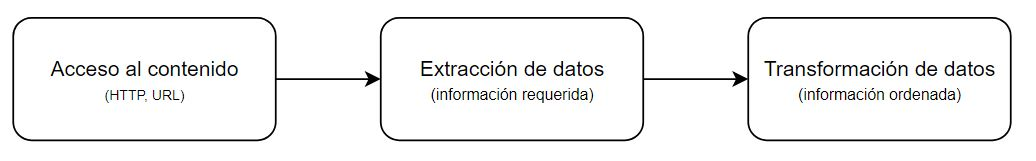
\includegraphics[width=6in]{web-scraping-phases.jpg}
\caption{Fases del web scraping}
\label{img:web-scraping-phases}
\end{figure}

Por otro lado, a lo largo del apéndice \ref{cha:funcionamiento basico de un web scraper}, se ilustra el
funcionamiento del agente software en cada una de las fases descritas anteriormente, así como de su
comportamiento con el servidor web al que se desea acceder.

\subsection{Herramientas software disponibles}
\label{subsec:herramientas software disponibles}
El software disponible que emplean los web scrapers puede dividirse en varios enfoques, ya sean bibliotecas
de programación de propósito general, frameworks, o entornos de escritorio.

Por lo general tanto los frameworks como los entornos de escritorio presentan una solución más sencilla
e integradora con respecto a bibliotecas de programación. Esto es debido a que ambos, no se ven afectados
a los posibles cambios HTML de los recursos a los que accede. Además, estas necesitan la integración de
otras múltiples bibliotecas adicionales para el acceso, análisis y extracción del contenido.

Este trabajo se desarrolla sobre bibliotecas de programación, las cuales se implementan como un programa
software convencional utilizando estructuras de control y de datos del propio lenguaje. Por lo general,
bibliotecas como \emph{curl \cite{curl-cran}} conceden acceso al sitio web deseado haciendo uso del
protocolo HTTP, mientras que los contenidos extraídos se analizan a través de funciones como la
coincidencia de expresiones regulares y la tokenización.

Comprender como las bibliotecas obtienen los datos de los sitios web, pasa por conocer las diferentes
formas en las que los documentos HTML se organizan. Existen dos técnicas, dependiendo si se realiza un
renderizado previo o no \cite{tfg-daniel-francisco-lopez}. La primera técnica consiste simplemente en
parsear, es decir, realizar un análisis léxico-sintáctico sobre estructuras XML o HTML. Se suele emplear
XPath o selectores CSS para su realización. Por otro, lado si es necesario que parte de la lógica del
sitio web pase al lado del cliente, este deberá pasar por un proceso de renderizado previo.

Con el paso del tiempo, cada vez se extiende más el uso de bibliotecas de desarrollo como JQuery, encargadas 
de pasan parte de la lógica del lado del servidor al lado del cliente con el objetivo de favorecer la 
interactividad. Estas páginas no podrán ser analizadas si no se renderizan antes.


\subsubsection{XPath}
\label{subsubsec:xpath}

\emph{XPath} es un lenguaje que permite construir expresiones que recorren y procesan un documento XML
\cite{xpath-wikipedia}. Puede utilizarse para navegar por documentos HTML, ya que este es un lenguaje
similar en cuanto a estructura a XML. \emph{XPath} es comúnmente utilizado en el web scraping para extraer
datos de documentos HTML, además utiliza la misma notación empleada en las URL para navegar por la
estructura del sitio web en cuestión.

\subsubsection{Selectores CSS}
\label{subsubsec:selectores CSS}

El segundo método de extracción de datos en documento HTML se realiza a través de lo que se conoce como
selectores CSS \cite{css-selectors-w3c}. CSS es el lenguaje utilizado para dar estilo a los documentos
HTML, por otro lado, los selectores son patrones que se utilizan para hacer coincidir y extraer elementos
HTML basados en sus propiedades CSS.

Hay múltiples sintaxis de selector diferentes, estas se corresponden con la forma en la que el documento
CSS está estructurado. En el fragmento de código \ref{cod:extraccion de datos de interes del documento}
se hace uso de los selectores \emph{'.text-primary'} y \emph{'.lister-item-header a'} para acceder al
contenido web deseado.

\subsection{Tipologias}
\label{subsec:tipologias}
Dependiendo de como se acceda y extraiga la información, existen dos técnicas de web scraping. Se mencionan
los siguientes supuestos a continuación:

\begin{itemize}
\item Si la información que se almacena no procede de sitios web concretos, sino que durante el análisis
de páginas web se encuentran enlaces que retroalimentan el análisis de otras nuevas, el método se conoce
como web crawling \cite{web-crawling-wikipedia}.

\item Si la información se extrae de sitios web concretos, donde ya se conoce como extraer y generar un
valor por la información, la técnica se conoce como web scraping genérico. Mientras que en el web crawling
el resultado de ejecución es la obtención de nuevas páginas, en el web scraping el resultado es la propia
información.
\end{itemize}

Es decir, la principal diferencia entre ambas, es que mientras los web scrapers extraen información de
páginas webs concretas, los web crawlers almacenan y acceden a las páginas a través de los enlaces
contenidos en las mismas. En la figura \ref{img:web-scraping-phases} se mostraba la arquitectura en fases
de un web scraper, veamos a continuación como es la arquitectura de un web crawler.

\begin{figure}[tphb]
\centering
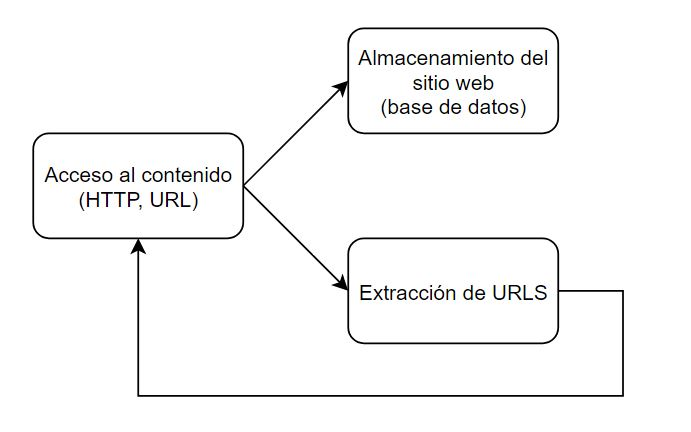
\includegraphics[width=4in]{web-crawler-phases.jpg}
\caption{Fases del web crawling}
\label{img:web-crawler-phases}
\end{figure}

Ya sea empleando cualquiera de estas dos tipologías, existen páginas que no pueden ser analizadas o
rastreadas. Esto es debido a que algunos sitios web solo están disponibles con una autorización previa, o
necesitan información especial para su acceso.

\section{Posibilidades prácticas del web scraping}
\label{sec:posibilidades practicas del web scraping}
Son muchas las aplicaciones prácticas de la minería web, la mayoría de estas entran en el ámbito de la
ciencia de los datos. En la siguiente lista se exponen algunos casos de su uso en la vida real
\cite{web-scraping-seppe}:

\begin{itemize}
\item Bancos y otras instituciones financieras utilizan minería web para analizar a la competencia.
Inversores también utilizan web scraping, para hacer un seguimiento de artículos de prensa relacionados
con los activos de su cartera.

\item En las redes sociales se emplea minería de datos para conocer la opinión de la gente a cerca de un
determinado tema.

\item Existen aplicaciones capaces de analizar diferentes sitios web y encontrar los mismos productos a
precio reducido. Incluso capaces de detectar ofertas de artículos a tiempo récord.

\item etcétera
\end{itemize}

El minado web contiene infinidad de aplicaciones, muy diversas e interesante capaces de automatizar el
trabajo y conseguir la información de forma ordenada.

No obstante, muchos sitios web ofrecen alternativas como el uso de APIs o ficheros estructuras para el
acceso a dichos datos. En general el web scraping es una técnica que consume bastantes recursos, por lo
que el desarrollador debe limitar su uso si existen otras alternativas, como las APIs, que proporcionan
los mismos resultados.

\section{Retos del web scraping}
\label{sec:retos del web scraping}
La forma en la que se crean los sistemas de extracción web se ha discutido desde diferentes perspectivas
a lo largo del tiempo. Se emplean métodos científicos como el aprendizaje automático, la lógica o el
procesamiento del lenguaje natural para lograr su implementación.

Uno de los principales retos a afrontar tiene relación con las fuentes cambiantes de información. A menudo,
una herramienta de extracción tiene que obtener datos de forma rutinaria de una determinada página o sitio
web que puede evolucionar con el tiempo. Estos cambios se producen sin previo aviso, son imprevisibles,
por lo que es bastante probable que los raspadores web se vean sometidos a cambios. Por ello, surge la
necesidad crear herramientas flexibles capaces de detectar y afrontar modificaciones estructurales de las
fuentes web relacionadas.

Otros problemas recaen sobre la información extraída. En primer lugar, uno de los aspectos que se deben
tener en cuenta al obtener información trata sobre la fiabilidad de la misma. Aunque la información
exista y se pueda ser analizada, esta puede que no sea correcta. La gramática y la ortografía pueden ser
un problema en la fase de análisis, ya que información puede perderse o ser falsamente recogida. Por otro
lado, tanto aplicaciones que tratan con datos personales, como software de minado deben ofrecer garantías
de privacidad. Por lo tanto, los posibles intentos de violar la privacidad del usuario deben ser
identificados y contrarrestados a tiempo y de forma adecuada.

Puesto que multitud de técnicas de minería web requieren ayuda humana, un primer reto consiste en
proporcionar un alto grado de automatización, reduciendo así al máximo el esfuerzo humano. Sin embargo,
la ayuda humana puede desempeñar un papel importante a la hora de elevar el nivel de precisión alcanzado
por un sistema de extracción de datos web, por ello la clave está en encontrar un equilibrio entre
automatización e intervención humana.

Por último, a pesar de que las herramientas de web scraping han evolucionado con el tiempo, los aspectos
legales están algo inexplorados pues dependen de los términos y condiciones de cada sitio web en cuestión.

\section{Aspectos ético-legales del web scraping}
\label{sec:aspectos etico-legales del web scraping}
Para comprender los aspectos legales del web scraping, debemos recordar el robot o agente software
definido en el apartado \ref{subsec:extraccion de los datos}. Este agente software,
previamente examinado por el servidor, es el que se encarga de acceder y realizar un recorrido por el
contenido web.

Durante el acceso al contenido, se espera que este agente se ajuste a los términos de uso del sitio en
cuestión, así como el cumplimiento del archivo \emph{'robots.txt'} \footnote{Archivo alojado en el
servidor web, que gestiona el tráfico del mismo e indica los documentos a los que no se debe acceder de
forma automática \cite{robots-txt}.}, con el objetivo de evitar accesos no deseados y sobrecargas en el
servidor.

Puesto que el documento \emph{'robots.txt'} no es de obligado cumplimiento, a lo largo de los años la
reputación del web scraping ha decrecido de forma significativa. Muchos agentes software no siguen las
indicaciones determinadas, por lo que definir la cantidad de accesos y archivos a los que se accede
dependerá de la ética de cada desarrollador.

Con el objetivo de tener una cierta garantía de que nuestro agente software cumple con los aspectos
ético-legales, se deben tener en consideración las siguientes cuestiones \cite{legalidad-web-scraping}:

\begin{itemize}
\item Leer los términos de uso de la página web en al que se vaya a realizar el minado.

\item Inspeccionar y cumplir con el documento robots.txt, para ser capaces de identificar los accesos
del servidor.

\item Realizar peticiones al servidor de forma controlada. Puede que el índice de solicitudes al servidor
no este especificado en el documento, si esto sucede debemos determinar un número de solicitudes razonable,
por ejemplo, una solicitud por segundo.
\end{itemize}


















\chapter{Paquetes de programación orientados al web scraping}
\label{cha:paquetes de programacion orientados al web scraping}

\section{Búsqueda de paquetes destinados al web scraping}
\label{sec:busqueda de paquetes destinados al web scraping}

Como se especificó en la sección \ref{sec:objetivo y limitaciones} este trabajo se limitará a realizar
una comparativa de los programas software de minado web más frecuentes. Esta comparativa se efectúa con el
fin de conocer cuál o cuáles de estos programas o paquetes software son los más rentables para este propósito.

¿Como saber que paquetes software destinados al minado web son los más comunes? Durante todo este capítulo
se procederá a la búsqueda, selección e introducción de programas software empleados para el web scraping. 
Cabe destacar que Python y R serán los lenguajes de programación con los que se trabajará tanto para el 
desarrollo de la herramienta de comparación, como para el proceso de extracción de datos.

El primer paso consiste en buscar todos los elementos posibles que conforman la población de paquetes
software del mercado, ya sean de Python o R. La búsqueda de estos paquetes se ha realizado a través de las 
distintas fuentes de información mostradas a continuación:

\begin{enumerate}
  \item GitHub \cite{github}. Gran parte de los desarrolladores de estos programas, publican su trabajo en
  estos repositorios de código abierto.
  \item CRAN \cite{cran}. The Comprehensive R Archive Network es una red de servidores ftp y web que
  almacena versiones idénticas de código y documentación para R.
  \item PyPi \cite{pypi}. Python Package Index es un repositorio de software para Python, útil para la
  búsqueda de paquetes de un determinado propósito.
\end{enumerate}

\section{Bibliotecas de Python encontradas durante el proceso de búsqueda}
\label{sec:bibliotecas de python encontradas durante el proceso de busqueda}

A continuación, se hará una breve sinopsis de los paquetes encontrados. Esta introducción tiene como
objetivo conocer el funcionamiento de los paquetes, cuáles son sus funciones y como es el proceso de
extracción. Es posible que algunos de los paquetes hayan sido desarrollados tanto en R como en Python. En 
ese caso, por un lado, la introducción se realzará de forma conjunta, sin embargo, será interesante ver 
el código del mismo en ambos casos y como se comportan estos ante los distintos test de evaluación.

\subsection{Beautiful Soup}
\label{subsec:beautiful soup}

\emph{Beautiful Soup} \cite{beautifulsoup} es una de las librerías de Python más comunes en el ámbito del
web scraping, está diseñada para extraer datos de documentos XML y HTML.

La técnica que emplea este algoritmo consiste en la creación de un árbol de análisis, donde se disponen
todos los elementos del documento como nodos del propio árbol. Una vez disponible, distintos analizadores 
pueden navegar, buscar y modificar este con el fin de obtener la mayor cantidad posible de información.

Beautiful Soup tiene a html.parse como analizador estándar de documentos HTML, pero también admite varios
analizadores de terceros. En la tabla \ref{tab:analizadores disponibles en beautiful soup} se muestran los 
distintos analizadores disponibles, así como un pequeño resumen de las ventajas y desventajas de estos.

\begin{table}[h]
  \begin{center}
  \begin{tabular}{| c | c | c | c |}
  \hline Tipo de analizador & Forma de uso & Ventajas & Desventajas \\ \hline
  html & bs(markup, "html.parser") & Notablemente rapido & Mas lento que lxml\\
  lxml html & 	bs(markup, "lxml") & Muy rapido & Dependencia de C\\
  lxml xml & bs(markup, "xml") & Muy rapido y soporta xml & Dependencia de C\\
  html5lib & bs(markup, "html5lib") & Analiza igual que un buscador & Muy lento\\ \hline
  \end{tabular}
  \caption{Analizadores disponibles en Beautiful Soup}
  \label{tab:analizadores disponibles en beautiful soup}
  \end{center}
\end{table}

El empleo de distintos analizadores supondrá una importancia menor si se aplica sobre documentos bien 
formados, pues la solución aportada presentará la misma estructura que el propio documento original. En 
caso contrario, el uso de diferentes analizadores creará diferentes soluciones para un mismo documento. 
Veamos algún ejemplo.

Se emplea el analizador lxml sobre un documento HTML sencillo pero con erratas. Vemos como la solución 
aportada propone la inclusión de nuevas etiquetas \emph{<head>} y \emph{<body>}, sin embargo, ¿qué ha 
ocurrido con la etiqueta \emph{<p>}?.

\begin{Schunk}
  \begin{Soutput}
    > BeautifulSoup("<a></p>", "lxml")
    # <html><body><a></a></body></html>
  \end{Soutput}
\end{Schunk}

En lugar de ignorar la etiqueta \emph{</p>}, el analizador html5lib la empareja con una etiqueta \emph{<p>}
de apertura. También añade una etiqueta <head> que el analizador lxml habia obviado.

\begin{Schunk}
  \begin{Soutput}
    > BeautifulSoup("<a></p>", "html5lib")
    # <html><head></head><body><a><p></p></a></body></html>
  \end{Soutput}
\end{Schunk}

Al igual que lxml, html.parse ignora la etiqueta de cierre \emph{</p>}. Podemos observar que este analizador 
ni siquiera intenta crear un documento HTML bien formado añadiendo etiquetas \emph{<html>} o \emph{<body>}.

\begin{Schunk}
  \begin{Soutput}
    > BeautifulSoup("<a></p>", "html.parser")
    # <a></a>
  \end{Soutput}
\end{Schunk}

Como vemos diferentes analizadores crearan diferentes soluciones en caso de que el documento a analizar
no este bien formado. Por ello, si deseamos analizar múltiples documentos de los que no conocemos su origen
o estructura sería deseable especificar el tipo de analizador con el fin del obtener la solución deseada.

En cuanto al proceso de extracción que se emplea en este algoritmo es sencillo. En primer lugar, el documento ya sea
HTML o XML se convierte al completo en caracteres Unicode. Tras ello se crea un árbol de objetos donde
cada uno de ellos representa una etiqueta o tag del documento HTML ('<body>, '<p>', ...). Finalmente, un 
analizador especificado por parámetro, recorre el árbol buscando las partes del mismo que se desean.

\begin{figure}[tphb]
  \centering
  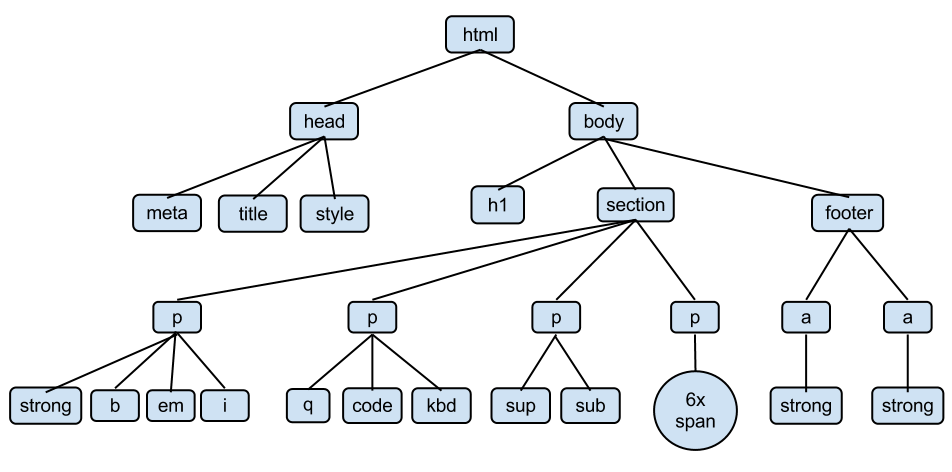
\includegraphics[width=4.5in]{bs-parse-tree.png}
  \caption{Arbol de objetos de Beautiful Soup\cite{bs-parse-tree}}
  \label{img:arbol de objetos de beautiful soup}
\end{figure}

Este algoritmo, no solo permite el recorrido automático del árbol en busca del texto del documento al
completo, sino que permite además la posibilidad de recorrer el mismo de forma manual, por lo que es posible
acceder a todos los objetos del árbol empleando métodos de navegación como \emph{soup.head, soup.parent,
soup.next\_sibling, ...}.

\subsection{JusText}
\label{subsec:justext}

\emph{JusText} \cite{justext} es una herramienta para eliminar el contenido repetitivo, como los enlaces 
de navegación, encabezados y pies de página de las páginas HTML. Está diseñado para preservar principalmente 
el texto que contiene frases completas.

La técnica que emplea este algoritmo consiste en lo que se conoce como segmentación. La idea es formar 
bloques de texto dividiendo la página HTML en etiquetas. Una secuencia de dos o más etiquetas como 
\emph{<br>}, \emph{<div>, ...}, separaría los bloques. 

Aunque no sea habitual, puede ocurrir que el contenido de estos bloques no sea homogéneo, es decir, que 
dentro de un mismo bloque haya una mezcla de información importante con contenido basura. La forma en la 
que JusText separa el contenido basura, denominado boilerplate, del contenido valioso se basa en el volumen 
de palabras con sentido gramatical. Aplicando esta heurística es posible hacer una distinción entre bloques 
como la que sigue:

\begin{itemize}
  \item Los bloques cortos que contienen un enlace son casi siempre del tipo boilerplate.
  \item Los bloques que contienen muchos enlaces son casi siempre del tipo boilerplate.
  \item Los bloques largos que contienen texto gramatical forman parte del contenido valioso, mientras que 
  todos los demás bloques largos son casi siempre del tipo boilerplate.
  \item Tanto los bloques buenos como los bloques de tipo boilerplate tienden a crear grupos, es decir,
  un bloque boilerplate suele estar rodeado de otros bloques de su mismo tipo y viceversa.
\end{itemize}

La dificultad real está en decidir cuando un texto es gramatical y cuando no. Aunque puede ser complicado,
JusText emplea una simple heurística basada en el volumen de palabras con sentido gramatical. Mientras que
un texto gramatical suele contener un cierto porcentaje de este tipo de palabras, como las listas y
enumeraciones, los contenidos de tipo boilerplate suelen carecer de ellas. En definitiva, los bloques
largos y algunos bloques cortos pueden clasificarse con una confianza muy alta. El resto de bloques cortos
pueden clasificarse observando los bloques circundantes.

Con el fin de facilitar el trabajo heurístico, JusText realiza un preprocesamiento del documento HTML. 
Durante esta fase, se elimina el contenido de las etiquetas \emph{<header>}, \emph{<style>} y \emph{<script>}. 
Ademas, el contenido de etiquetas como \emph{<select>} se clasifica inmediatamente como tipo boilerplate. 
Lo mismo ocurre con los bloques que contienen el símbolo de copyright ©.

Tras el proceso de segmentación y preprocesamiento se procede a la clasificación de bloques, donde a cada
uno de estos bloques se le asigna una clase dependiendo de su naturaleza:

\begin{enumerate}
  \item Malo: bloques de tipo boilerplate.
  \item Bueno: bloques pertenecientes al contenido principal.
  \item Corto: bloques demasiado cortos para tomar una decision sobre su naturaleza.
  \item Casi bueno: bloques intermedios entre cortos y buenos.
\end{enumerate}

¿Qué algoritmo sigue JusText para determinar esta clasificación? En el fragmento de código
\ref{cod:justext - algoritmo de clasificacion} se muestra cuál es el proceso de dicha clasificación 
para cada una de los cuatro tipos distintos de bloques. 

\begin{codefloat}
  \inputencoding{latin1}
  \lstinputlisting[style=CppExample]{scripts/clasificacion-justext.py}
  \inputencoding{utf8}
  \caption{JusText - Algoritmo de clasificación}
  \label{cod:justext - algoritmo de clasificacion}
\end{codefloat}

Podemos observar que se definen dos tipos de variables, la densidad y la longitud. Mientras que la longitud 
es el número de caracteres de bloque, la densidad se define como la proporción de caracteres o palabras 
dentro de una una etiqueta de tipo \emph{<a>}, o una lista de parada.

El algoritmo toma como parámetros dos enteros definidos como LENGTH\_LOW(70) y LENGTH\_HIGH(200), ademas 
de tres números de coma flotante, MAX\_LINK\_DENSITY(0.2), STOPWORDS\_LOW(0.3) y STOPWORDS\_HIGH(0.32). 
Los dos primeros establecen los umbrales para dividir los bloques por su longitud en tres tipos, cortos, 
medianos y largos. Los dos últimos dividen los bloques por la densidad de palabras de parada en bajos, 
medianos y altos.

La distinción entre bloques es muy sencilla, hasta ahora JusTest ha sido capaz de clasificar los bloques
buenos y malos, pero ¿qué ocurre con los bloques cortos y los bloques casi buenos? JusText reclasifica
este tipo de bloques en función de los bloques circundantes. Los bloques ya clasificados como buenos o
malos sirven como piedras base en esta etapa y su clasificación se considera fiable, por lo que nunca se
modifica. Esta reclasificación se puede ver resumida en la imagen \ref{img:justext - reclasificacion de
bloques}.

\begin{figure}[tphb]
  \centering
  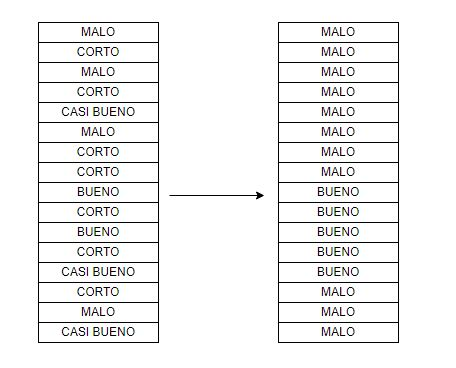
\includegraphics[width=4in]{justext-blocks-classification.jpg}
  \caption{JusText - Reclasificación de bloques}
  \label{img:justext - reclasificacion de bloques}
\end{figure}

La idea que subyace a la reclasificación es que los bloques 'boilerplate' suelen estar rodeados de otros 
bloques 'boilerplate' y viceversa. Los bloques casi buenos suelen contener datos útiles del corpus si se 
encuentran cerca de bloques buenos. Los bloques cortos suelen ser útiles sólo si están rodeados de bloques 
buenos por ambos lados.

\subsection{Inscriptis}
\label{subsec:inscriptis}

\emph{Inscriptis} \cite{inscriptis} es una biblioteca de conversión de HTML a texto basada en Python. Esta
librería es especialmente adecuada para aplicaciones que requieran representaciones de texto con una alta
precisión y calidad del contenido HTML.

A diferencia de otros algoritmos de extracción Inscriptis no solo tiene en cuenta el texto extraído, sino
que además la estructura del mismo es muy importante, por lo que este texto extraído podría acercarse más 
al obtenido por cualquier navegador web. 

Veamos una pequeña comparación entre la extracción de texto de Beautiful Soup \ref{subsec:beautiful soup}, 
con la extracción de texto de Inscriptis, donde se tiene un fragmento HTML como el siguiente, como objeto 
de prueba.

\begin{Schunk}
  \begin{Soutput}
    <ul>
        <li>first</li>
        <li>second</li>
    <ul>
  \end{Soutput}
\end{Schunk}

Si aplicásemos Beautiful Soup sobre este fragmento HTML el texto extraído sería algo como \emph{'firstsecond'},
donde no se tiene en cuenta el diseño ni la estructura del documento. Sin embargo, si aplicamos Inscriptis
sobre el mismo fragmento HTML, la salida obtenida sería la siguiente:

\begin{Schunk}
  \begin{Soutput}
    * first
    * second
  \end{Soutput}
\end{Schunk}

Inscriptis, no solo admite construcciones tan simples como la anterior, permite analizar construcciones 
mucho más complejas, como las tablas anidadas, y subconjuntos de atributos HTML y CSS donde es esencial 
una conversión precisa de HTML a texto.

La técnica que emplea Inscriptis se conoce como reglas de anotación, es decir, mapeos que permiten anotar 
el texto extraído. Estas anotaciones se basan en la información estructural y semántica codificada en las 
etiquetas y atributos HTML utilizados para controlar la estructura y diseño del documento original. 

Con el fin de asignar etiquetas y/o atributos HTML a las anotaciones, se emplea un algo parecido a un 
diccionario. En el diccionario mostrado a continuación, la etiqueta \emph{<h1>} produce las anotaciones 
heading y h1, una etiqueta \emph{<div>} con una clase que contiene el valor toc da como resultado la 
anotación table-of-contents, y todas las etiquetas con un atributo cite se anotan con citation.

\begin{Schunk}
  \begin{Soutput}
    {
      "h1": ["heading", "h1"],
      "h2": ["heading", "h2"],
      "b": ["emphasis"],
      "div#class=toc": ["table-of-contents"],
      "#class=FactBox": ["fact-box"],
      "#cite": ["citation"]
    }
  \end{Soutput}
\end{Schunk}

Imaginemos que se dispone de un documento HTML como el que sigue y unas reglas de anotación determinadas.

\begin{Schunk}
  \begin{Soutput}
    <h1>Chur</h1>
    <b>Chur</b> is the capital and largest town of the Swiss canton of the Grisons 
    and lies in the Grisonian Rhine Valley.
  \end{Soutput}
\end{Schunk}

En este ejemplo, la salida habitual según el diccionario anterior debería ser una etiqueta de cabecera y
otra de énfasis, veamos la salida que proporciona el proceso de asignación.

\begin{Schunk}
  \begin{Soutput}
    {"text": "Chur\n\nChur is the capital and largest town of the Swiss canton
          of the Grisons and lies in the Grisonian Rhine Valley.",
    "label": [[0, 4, "heading"], [0, 4, "h1"], [6, 10, "emphasis"]]}
  \end{Soutput}
\end{Schunk}

Como era de esperar la obtención del texto es precisa, pero no solo del texto sino de su estructura. Además,
la asignación de etiquetas también se ha realizado de forma correcta.

\subsection{Goose3}
\label{subsec:goose3}

\emph{Goose} \cite{goose3} es una librería de programación cuyo objetivo es la extracción de texto en 
artículos. Inicialmente, el proyecto fue iniciado con Java, pero han surgido nuevas versiones en diferentes 
lenguajes de programación como Scala o Python.

El objetivo del software es tomar cualquier artículo de noticias o página web de tipo artículo y no solo
extraer lo que es el cuerpo principal, sino también se extraen todos los metadatos e imágenes del mismo.
Goose extraerá: (1) texto principal del artículo, (2) imagen principal del artículo, (3) videos introducidos
en el artículo, (4) descripción y (5) meta tags.

La técnica que emplea Goose3 para la extracción de texto es muy similar a la que se emplea en Beautiful Soup
\ref{subsec:beautiful soup}, donde un árbol se recorre con el fin de obtener la mayor cantidad de información
valiosa posible.

\begin{codefloat}
  \inputencoding{latin1}
  \lstinputlisting[style=CppExample]{scripts/extraccion-goose3.py}
  \inputencoding{utf8}
  \caption{Goose3 - Algoritmo de extracción}
  \label{cod:goose3 - algoritmo de extraccion}
\end{codefloat}

Si observamos el algoritmo \ref{cod:goose3 - algoritmo de extraccion}, si se determina que en un cierto
nodo del árbol contiene texto, se crea un nuevo nodo y este se inserta en una lista. Con este proceso
todos los nodos que contienen información valiosa son agrupados y almacenados para su posterior uso.

Al igual que con Beautiful Soup, Goose puede emplear distintos analizadores, html de lxml o el conocido como
soup parser de lxml. Pero no solo es posible configurar el analizador, también se puede determinar el agente
de usuario que se empleará para la extracción.

\begin{Schunk}
  \begin{Soutput}
    > g = Goose({'browser_user_agent': 'Mozilla', 'parser_class':'soup'})
  \end{Soutput}
\end{Schunk}

\subsection{News-please}
\label{subsec:news-please}

\emph{News-please} \cite{news-please} es un web scraper y web crawler de código abierto escrito en Python
desarrollado para cumplir cinco requisitos: (1) extracción de noticias de cualquier sitio web, (2) extracción
completa del sitio web, (3) alta calidad de la información extraída, (4) facilidad de uso y (5) mantenibilidad.

A diferencia de otros web scrapers ya mencionados anteriormente, news-please emplea herramientas ya existentes,
las cuales se amplían con nuevas funcionalidades con el objetivo de cumplir con los requisitos señalados.

\begin{figure}[tphb]
  \centering
  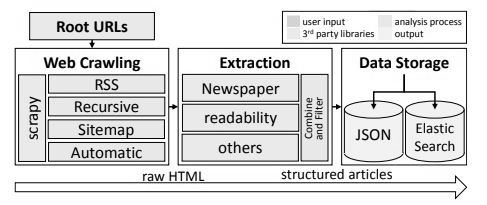
\includegraphics[width=4.5in]{newsplease-processing.jpg}
  \caption{News-please - Proceso de scraping y crawling}
  \label{img:news-please - proceso de scraping y crawling}
\end{figure}

En cuanto al proceso de web crawling, news-please lo divide en dos subtareas, en primer lugar se descarga 
el documento HTML empleando el framework \emph{Scrapy}. En segundo lugar, con el objetivo de encontrar 
todos los artículos publicados en dicho documento se admiten cuatro técnicas:

\begin{enumerate}
  \item RSS \footnote{formato XML para distribuir contenido en la web}: análisis de los canales RSS para 
  encontrar los artículos recientes.
  \item Recursiva: seguimiento de los enlaces enlaces internos en las páginas rastreadas.
  \item Sitemap \footnote{Un sitemap es un archivo que enumera las URL visibles de un determinado sitio, 
  el objetivo principal es revelar dónde pueden buscar contenido las máquinas.}: analiza los sitemaps en 
  busca de enlaces a todos los artículos.
  \item Automático: prueba los sitemaps, vuelve a ser recursivo en caso de error.
\end{enumerate}

Estos cuatro enfoques también pueden combinarse, por ejemplo, iniciando dos instancias de news-please en 
paralelo, una en modo automático para obtener todos los artículos publicados hasta el momento y otra 
instancia en modo RSS para recuperar los artículos recientes.

Para el proceso de web scraping, se emplean herramientas ya existentes en el mercado con el objetivo de 
obtener la información deseada, es decir, título, párrafo principal, contenido principal, autor, fecha e 
imagen principal. Por un lado, news-please ha decidido utilizar herramientas como \emph{Newspaper} 
\ref{subsec:news-paper} o \emph{Readability} \ref{subsec:readability} para el proceso de extracción del 
contenido principal en artículos, mientras que por otro se emplea \emph{Regex} para la extracción de fechas 
de publicación.

\subsection{Trafilatura}
\label{subsec:trafilatura}

\emph{Trafilatura} \cite{trafilatura} es un paquete de Python que descarga, analiza y extrae datos de páginas
web. Combina dos bibliotecas de web scraping ya existentes, \emph{Readability} \ref{subsec:readability} y
\emph{JusText} \ref{subsec:justext} como redes de seguridad y fallbacks.

La técnica que emplea el algoritmo de extracción de este paquete se fundamenta en una cascada de filtros
basados en reglas y heurística de contenido. Veremos que al igual que muchos otros algoritmos de extracción,
usa los árboles de objetos como estructura de datos.

En primer lugar, se realiza lo que se conoce como delimitaciones de contenido, donde mediante expresiones
XPath dirigidas y atributos HTML comunes, se excluyen partes no deseadas del código HTML creando un árbol
de objetos. Las mismas operaciones se realizan para los comentarios en caso de que formen parte de la
extracción.

\begin{codefloat}
  \inputencoding{latin1}
  \lstinputlisting[style=CppExample]{scripts/delimitacion-trafilatura.py}
  \inputencoding{utf8}
  \caption{Trafilatura - Delimitación de contenido}
  \label{cod:trafilatura - delimitacion de contenido}
\end{codefloat}

Si se detecta que la extracción realizada ha sido posiblemente defectuosa, se ejecuta lo que se conocen 
como algoritmos de respaldo. Estos aplican una heurística basada en la longitud de las líneas, la relación 
texto/marcado y la posición/profundidad de los elementos en el árbol HTML. Una vez aplicados estos 
algoritmos, su resultado se compara con la extracción 'casera' y se determina la extracción más eficaz, 
sobre todo en términos de longitud e impurezas.

Por último, es caso de que ambas soluciones provoquen una salida defectuosa, se ejecuta una extracción base
con el fin de buscar elementos de texto 'salvajes' que probablemente se hayan pasado por alto. Esto implica
la búsqueda de cualquier elemento con contenido textual útil.

\begin{codefloat}
  \inputencoding{latin1}
  \lstinputlisting[style=CppExample]{scripts/respaldo-trafilatura.py}
  \inputencoding{utf8}
  \caption{Trafilatura - Algoritmo de respaldo y extraccion base}
  \label{cod:trafilatura - algoritmo de respaldo}
\end{codefloat}

Como resultado de toda esta consecucion de algoritmos se obtienen los textos principales y los posibles 
comentarios de los documento HTML analizados, con la posibilidad de conservar elementos estructurales como
párrafos, títulos, listas, comillas, código, saltos de línea, formato de texto en línea... En la extraccion, 
también se incluyen metadatos, es decir, título, nombre del sitio, autor, fecha, categorías y etiquetas.

\subsection{Dragnet}
\label{subsec:dragnet}

\emph{Dragnet} \cite{dragnet} es un web scraper escrito en Python y construido sobre el entorno de cálculo
numérico 'numpy/scipy/Cython'. Como hemos visto hasta ahora, el objetivo de cualquier algoritmo de
extracción es separar el contenido principal del contenido de navegación, los bloques de publicidad, los
avisos de copyright y similares en las páginas web. La mayoría de estos algoritmos emplean heurísticas
determinas para este fin. Dragnet se encarga de realizar esta separación de contenido empleando el
aprendizaje automático.

El algoritmo comienza dividiendo el documento HTML en una secuencia de bloques utilizando el DOM 
\footnote{El DOM define la manera en que objetos y elementos se relacionan entre sí en el navegador y en 
el documento. \cite{dom-wikipedia}} y un conjunto específico de etiquetas como \emph{<div>}, \emph{<p>} o
\emph{<h1>}, que modifican la estructura del propio documento. Iterando por el DOM, cada vez que el algoritmo 
se encuentra alguna de las etiquetas mencionadas anteriormente, se crea un nuevo bloque. Aquellos bloques
sin contenido de valor, son descartados. 

Una vez separado el documento en bloques, se deben asignar un conjunto de características a cada uno. Estas 
serán útiles en un clasificador con el objetivo de predecir el contenido con valor, del contenido 
'boilerplate' a nivel de bloque. Cualquier bloque con más del 10\% de los tokens extraídos se etiqueta 
como contenido valioso.

La primera característica consiste en la densidad de texto y enlaces. La intuición es que los bloques de 
contenido tienen una mayor densidad de texto y una menor densidad de enlaces que los bloques denominados 
boilerplate, ya que muchos de estos ultimos son bloques que consisten en breves fragmentos de palabras o 
son principalmente texto ancla. 

El segundo tipo de característica está diseñada heurísticamente para capturar información semántica en el
código HTML que dejan los programadores. Muchos atributos como \emph{id} o \emph{class}, y etiquetas HTML 
incluían tokens tipo \emph{comment}, \emph{header} y \emph{nav}. Estos nombres descriptivos son utilizados 
por los programadores cuando escriben CSS y Javascript y, puesto que se eligen con el objetivo de que tengan 
sentido para el programador, incorporan cierta información semántica sobre el contenido del bloque.

\begin{table}[h]
  \begin{center}
  \begin{tabular}{| c | c | c | c |}
  \hline Token & Content : No Content & Percent of blocks  \\ \hline
  menu & 1 : 372.6 & 2.2\% \\
  widget & 1 : 314.1 & 4.6\% \\
  nav & 1 : 68.9 & 3.3\% \\
  facebook & 1 : 18.3 & 1.3\% \\
  top & 1 : 13.3 & 1.9\% \\
  twitter & 1 : 8.5 & 2.3\% \\
  title & 1 : 3.3 & 10.5\% \\
  header & 1 : 2.9 & 3.7\% \\ \hline
  comment & 3.2 : 1 & 21.3\% \\
  author & 4.9 : 1 & 7.9\% \\
  thread & 5.0 : 1 & 3.0\% \\
  avatar & 42.1 : 1 & 3.2\% \\ \hline
  \end{tabular}
  \caption{Comparación de tokens en el atributo \emph{class}}
  \label{tab:Comparacion de tokens en el atributo class}
  \end{center}
\end{table}

En la tabla \ref{tab:Comparacion de tokens en el atributo class} se enumeran algunos tokens seleccionados
en el atributo de clase junto con sus ratios de probabilidad de contenido y no contenido. Los tokens de la
parte superior de la tabla tienen más probabilidades de aparecer en bloques sin contenido, mientras que los
de la parte inferior tienen más probabilidades de aparecer en bloques con contenido. Para una mejor 
visualización, se forman dos grupos, según estén asociados a bloques de no contenido o de contenido.

Finalmente, la tercera característica incluye varias ideas. Por un lado, la relación entre la longitud del 
texto y el número de etiquetas HTML tiende a ser mayor en los bloques de contenido. En segundo lugar, las 
secciones de la página que no son de contenido tienden a estar agrupadas, de modo que la diferencia en la 
proporción de contenido y etiquetas de un bloque a otro tiende a ser pequeña en las regiones que no son de 
contenido. La idea final es combinar la proporción de etiquetas de contenido y la diferencia en la 
proporción de etiquetas de contenido en un enfoque de agrupación de k-means no supervisado, de modo que 
los bloques sin contenido se agrupen naturalmente cerca del origen.

\subsection{Readability}
\label{subsec:readability}

\subsection{HTML-Text}
\label{subsec:html-text}

\emph{HTML-Text} \cite{html-text} es una librería software destinada a la extracción de texto en documentos
HTML. Las principales diferencias entre emplear expresiones XPath \emph{.xpath('//text()')} o emplear
otros algoritmo de extracción como Beautiful Soup \emph{.get\_text()} son: (1) Por un lado, el texto extraído
es limpio, ya que no contiene estilos en línea, javascript o comentarios los normalmente no son visibles 
para los usuarios, (2) en segundo lugar, se normalizan los espacios en blanco de una forma más inteligente 
que empleando \emph{.xpath('normalize-space())}, (3) por último, se añaden nuevas líneas para que el texto 
de salida se parezca más a cómo se representa en los navegadores. 

\subsection{Newspaper3k}
\label{subsec:news-paper}

\section{Paquetes de R encontrados durante el proceso de búsqueda}
\label{sec:paquetes de r encontrados durante el proceso de busqueda}

\section{Paquetes seleccionados para el proceso de análisis}
\label{sec:paquetes seleccionados para el proceso de analisis}

\chapter{Selección de variables de análisis y proceso de estudio}
\label{cha:seleccion de variables de analisis y proceso de estudio}

% Optional in PFCs
%
\chapter{Pliego de condiciones}
\label{cha:pliego-de-condiciones}

Blah, blah, blah.

%%% Local Variables:
%%% TeX-master: "../book"
%%% End:


%Obligatorio en TFGs
\chapter{Conclusiones y futuras líneas de trabajo}
\label{cha:conclusiones y futuras lineas de trabajo}

%
% Fin de la seccion de capitulos
%%%%%%%%%%%%%%%%%%%%%%%%%%%%%%%%%%%%%%%%%%%%%%%%%%%%%%%%%%%%%%%%%%%%%%%%%%%
%%%%%%%%%%%%%%%%%%%%%%%%%%%%%%%%%%%%%%%%%%%%%%%%%%%%%%%%%%%%%%%%%%%%%%%%%%%


%%%%%%%%%%%%%%%%%%%%%%%%%%%%%%%%%%%%%%%%%%%%%%%%%%%%%%%%%%%%%%%%%%%%%%%%%%%
%
% Generic template for TFC/TFM/TFG/Tesis
%
% $Id: bibliography.tex,v 1.9 2015/06/05 00:10:32 macias Exp $
%
% By:
%  + Javier Macías-Guarasa. 
%    Departamento de Electrónica
%    Universidad de Alcalá
%  + Roberto Barra-Chicote. 
%    Departamento de Ingeniería Electrónica
%    Universidad Politécnica de Madrid   
% 
% Based on original sources by Roberto Barra, Manuel Ocaña, Jesús Nuevo,
% Pedro Revenga, Fernando Herranz and Noelia Hernández. Thanks a lot to
% all of them, and to the many anonymous contributors found (thanks to
% google) that provided help in setting all this up.
%
% See also the additionalContributors.txt file to check the name of
% additional contributors to this work.
%
% If you think you can add pieces of relevant/useful examples,
% improvements, please contact us at (macias@depeca.uah.es)
%
% You can freely use this template and please contribute with
% comments or suggestions!!!
%
%%%%%%%%%%%%%%%%%%%%%%%%%%%%%%%%%%%%%%%%%%%%%%%%%%%%%%%%%%%%%%%%%%%%%%%%%%%

%\bibliographystyle{plainnat}
%\bibliographystyle{dinat}
%\bibliographystyle{unsrt}
\bibliographystyle{IEEEtran}

% The following is overly complicated because I was not able to do so in
% another way. The problem is the bibliography command being "called"
% from both the root and anteproyecto directories...
%
% Here define as many bibfiles as needed
\newcommand{\mybibfileOne}{biblio/biblio.bib}
%\newcommand{\mybibfileTwo}{biblio/biblio2.bib}
%...
%\newcommand{\mybibfileN}{biblio/biblioN}

% This is for a single bib file
\newcommand{\mybibfiles}{\myreferencespath\mybibfileOne}
% but do this for multiple files
%\newcommand{\mybibfiles}{\myreferencespath\mybibfile1,\myreferencespath\mybibfile2,...,\myreferencespath\mybibfileN}

% Do not touch this
\inputencoding{latin1}
\bibliography{\mybibfiles}
\inputencoding{utf8}

%%% Local Variables:
%%% TeX-master: "../book"
%%% coding: utf-8
%%% End:


 % Bibliografia


%%%%%%%%%%%%%%%%%%%%%%%%%%%%%%%%%%%%%%%%%%%%%%%%%%%%%%%%%%%%%%%%%%%%%%%%%%%
% Comienzo de apendices
%                                 

\begin{appendices}
  \chapter{Funcionamiento básico de un web scraper}
\label{cha:funcionamiento basico de un web scraper}

Siguiendo las directrices determinadas en la sección \ref{subsec:extraccion de los datos}, se
muestra el funcionamiento de un web scraper durante las tres fases definidas. Para ello se realizará un
pequeño ejemplo mostrando el comportamiento del mismo y de como interactúa con el servidor web al que
se desea acceder.

Para el desarrollo de este ejemplo se han empleado bibliotecas software basadas en el lenguaje de
programación R, capaces de extraer datos de cualquier web. En este caso la web sujeta al análisis será,
\emph{imdb} encargada de asignar un ranking entre películas y series.

\section{Fase de búsqueda}
\label{sec:fase de busqueda}

Antes de comenzar con la primera de las tres etapas, debemos asegurarnos que nuestro agente software
cumple con todos los aspectos ético-legales descritos en la sección \ref{sec:aspectos etico-legales del web
scraping}. Los términos y servicios de la página deberán ser leídos, al igual que el documento
\emph{'robots.txt'} con el objetivo de conocer cuáles son los accesos disponibles y el índice de solicitudes
a realizar.

En el fragmento de código \ref{cod:solicitud del documento robots.txt} se muestra la solicitud al servidor
realizada. A través de la biblioteca \emph{robotstxt} \cite{robotstxt-cran} y haciendo uso de la función
\emph{get\_robotstxt} se obtiene el documento deseado.

Es posible que la solicitud del documento no se realice correctamente, pues o bien la página no dispone
del documento en ese instante, o la función ha fallado durante su solicitud. En cualquiera de estos dos
escenarios, es posible realizar una doble comprobación accediendo al mismo a través de la propia URL,
\emph{https://www.imdb.com/robots.txt}.

\begin{codefloat}
\inputencoding{latin1}
\lstinputlisting[style=CppExample]{appendix/ejemplo-basico-web-scraping-1.R}
\inputencoding{utf8}
\caption{Solicitud del documento \emph{robots.txt}}
\label{cod:solicitud del documento robots.txt}
\end{codefloat}

\begin{Schunk}
\begin{Soutput}
# robots.txt for https://www.imdb.com properties
User-agent: *
Disallow: /OnThisDay
Disallow: /ads/
Disallow: /ap/
Disallow: /mymovies/
Disallow: /r/
Disallow: /register
Disallow: /registration/
...
\end{Soutput}
\end{Schunk}


Una vez se ha accedido al documento \emph{'robots.txt'}, conociendo los posibles accesos al servidor, y
determinando el número de solicitudes máximas por segundo, es posible acceder y descargar el fichero
HTML de forma segura. Para este propósito se empleará la función \emph{read\_html} de la biblioteca
\emph{xml2} \cite{xml2-cran} la cual se detalla a continuación.

\begin{codefloat}
\inputencoding{latin1}
\lstinputlisting[style=CppExample]{appendix/ejemplo-basico-web-scraping-2.R}
\inputencoding{utf8}
\caption{Acceso y descarga del archivo HTML}
\label{cod:acceso y descarga del archivo html}
\end{codefloat}

El valor que retorna la función \emph{read\_html}, se trata del archivo HTML integro, donde se incluyen
cabecera, cuerpo y demás etiquetas del mismo. Una vez que se dispone de la página, es posible comenzar
con la extracción de datos de interés de la misma.

\section{Fase de extracción}
\label{sec:fase de extraccion}

Para el minado se empleará \emph{rvest} \cite{rvest-cran}, una de las bibliotecas software más comunes en
este aspecto, diseñada para trabajar con \emph{magrittr} \cite{magrittr-cran} y facilitar tareas de la
extracción. Además, será necesario el uso de funciones como \emph{html\_nodes()} y \emph{html\_text()}.

Durante esta fase de extracción se obtendrán tanto los títulos como el ranking asignado a cada película o
serie. Para realizar la extracción de forma correcta, se deberá conocer la etiqueta HTML que envuelve dicha
información.

\begin{codefloat}
\inputencoding{latin1}
\lstinputlisting[style=CppExample]{appendix/ejemplo-basico-web-scraping-3.R}
\inputencoding{utf8}
\caption{Extracción de datos de interés del documento}
\label{cod:extraccion de datos de interes del documento}
\end{codefloat}

\begin{Schunk}
\begin{Soutput}
[1] "1." "2." "3." "4." "5." "6."

[1] "Animales nocturnos"   "Train to Busan"       "La llegada (Arrival)"
[4] "Escuadrón suicida"    "Deadpool"             "Hush (Silencio)"     
\end{Soutput}
\end{Schunk}


\section{Fase de transformación}
\label{sec:fase de transformacion}

Una vez los datos han sido extraídos, la última fase consiste en la transformación de los mismos. Los datos
desordenados deberán ser convertidos en estructuras de datos ordenadas y coherentes con el fin su posible
almacenamiento en una base de datos.

\begin{codefloat}
\inputencoding{latin1}
\lstinputlisting[style=CppExample]{appendix/ejemplo-basico-web-scraping-4.R}
\inputencoding{utf8}
\caption{Transformación de datos en un data frame}
\label{cod:transformacion de datos en un data frame}
\end{codefloat}

\begin{Schunk}
\begin{Soutput}
  Rank                Title
1   1.   Animales nocturnos
2   2.       Train to Busan
3   3. La llegada (Arrival)
4   4.    Escuadrón suicida
5   5.             Deadpool
6   6.      Hush (Silencio)
\end{Soutput}
\end{Schunk}


Una vez los datos han sido ordenados en una estructura de datos propia, en este caso un data frame, es
posible trabajar con ellos de forma más cómoda y sencilla.








\end{appendices}

%
% Fin de apendices
%%%%%%%%%%%%%%%%%%%%%%%%%%%%%%%%%%%%%%%%%%%%%%%%%%%%%%%%%%%%%%%%%%%%%%%%%%%

\backmatter

%%%%%%%%%%%%%%%%%%%%%%%%%%%%%%%%%%%%%%%%%%%%%%%%%%%%%%%%%%%%%%%%%%%%%%%%%%%
%
% Generic template for TFC/TFM/TFG/Tesis
%
% $Id: backpage.tex,v 1.6 2018/12/12 15:29:21 macias Exp $
%
% By:
%  + Javier Macías-Guarasa. 
%    Departamento de Electrónica
%    Universidad de Alcalá
%  + Roberto Barra-Chicote. 
%    Departamento de Ingeniería Electrónica
%    Universidad Politécnica de Madrid   
% 
% Based on original sources by Roberto Barra, Manuel Ocaña, Jesús Nuevo,
% Pedro Revenga, Fernando Herránz and Noelia Hernández. Thanks a lot to
% all of them, and to the many anonymous contributors found (thanks to
% google) that provided help in setting all this up.
%
% See also the additionalContributors.txt file to check the name of
% additional contributors to this work.
%
% If you think you can add pieces of relevant/useful examples,
% improvements, please contact us at (macias@depeca.uah.es)
%
% You can freely use this template and please contribute with
% comments or suggestions!!!
%
%%%%%%%%%%%%%%%%%%%%%%%%%%%%%%%%%%%%%%%%%%%%%%%%%%%%%%%%%%%%%%%%%%%%%%%%%%%

%%%%%%%%%%%%%%%%%%%%%%%%%%%%%%%%%%%%%%%%%%%%%%%%%%%%%%%%%%%%%%%%%%%%%%%%%%%
% Right now (november 2013), it's only defined for TFGs at UAH
%%%%%%%%%%%%%%%%%%%%%%%%%%%%%%%%%%%%%%%%%%%%%%%%%%%%%%%%%%%%%%%%%%%%%%%%%%%

\ifthenelse{\equal{\mybookworktype}{TFG}}
{
  %%%%%%%%%%%%%%%%%%%%%%%%%%%%%%%%%%%%%%%%%%%%%%%%%%%%%%%%%%%%%%%%%%%%%%%%%%%
%
% Generic template for TFC/TFM/TFG/Tesis
%
% $Id: backpage-tfg-uah.tex,v 1.10 2015/06/05 00:10:33 macias Exp $
%
% By:
%  + Javier Macías-Guarasa. 
%    Departamento de Electrónica
%    Universidad de Alcalá
%  + Roberto Barra-Chicote. 
%    Departamento de Ingeniería Electrónica
%    Universidad Politécnica de Madrid   
% 
% Based on original sources by Roberto Barra, Manuel Ocaña, Jesús Nuevo,
% Pedro Revenga, Fernando Herránz and Noelia Hernández. Thanks a lot to
% all of them, and to the many anonymous contributors found (thanks to
% google) that provided help in setting all this up.
%
% See also the additionalContributors.txt file to check the name of
% additional contributors to this work.
%
% If you think you can add pieces of relevant/useful examples,
% improvements, please contact us at (macias@depeca.uah.es)
%
% You can freely use this template and please contribute with
% comments or suggestions!!!
%
%%%%%%%%%%%%%%%%%%%%%%%%%%%%%%%%%%%%%%%%%%%%%%%%%%%%%%%%%%%%%%%%%%%%%%%%%%%

% This is a trick to avoid the header to be shown. There must be a
% better way...
\chapter*{ }
\thispagestyle{empty}

\cleartoleftpage
\thispagestyle{empty}

% To add background watermark, defined in config/preamble.tex
\BgThispage

% Nice example of tikz
% \begin{tikzpicture}[remember picture,overlay]
%   \node [xshift=1cm,yshift=1cm] at (current page.south west)
%   [text width=7cm,fill=red,red!20,rounded corners,above right]
%   {
%     This is an absolutely positioned text in the
%     lower left corner. No shipout-hackery is used.
%   };
% \end{tikzpicture}

\begin{tikzpicture}[remember picture,overlay]
    \node[yshift=-5cm] at (current page.north west)
      {
        \begin{tikzpicture}[remember picture, overlay]
          \draw[fill=headingPortadaTFG,headingPortadaTFG] (0,0) rectangle (\paperwidth,5cm);

          \node [yshift=3cm, xshift=0.5\paperwidth, font=\Huge, text centered, midway] {\color{textoHeadingPortadaTFG}\mybookuniversity};
          \node [yshift=2cm, xshift=0.5\paperwidth, font=\Huge, text centered, midway] {\color{textoHeadingPortadaTFG}\mybookschool};

        \end{tikzpicture}
      };
   \end{tikzpicture}


\large
\vspace{20cm}
\begin{center}
  
  \centerline{
\includegraphics[height=2.5cm]{uah/01_logo-vA_pant293.pdf}}

\end{center}



%%% Local Variables:
%%% TeX-master: "../book"
%%% End:



}
{
\ifthenelse{\equal{\mybookworktype}{TFM}}
{
  %%%%%%%%%%%%%%%%%%%%%%%%%%%%%%%%%%%%%%%%%%%%%%%%%%%%%%%%%%%%%%%%%%%%%%%%%%%
%
% Generic template for TFC/TFM/TFG/Tesis
%
% $Id: backpage-tfg-uah.tex,v 1.10 2015/06/05 00:10:33 macias Exp $
%
% By:
%  + Javier Macías-Guarasa. 
%    Departamento de Electrónica
%    Universidad de Alcalá
%  + Roberto Barra-Chicote. 
%    Departamento de Ingeniería Electrónica
%    Universidad Politécnica de Madrid   
% 
% Based on original sources by Roberto Barra, Manuel Ocaña, Jesús Nuevo,
% Pedro Revenga, Fernando Herránz and Noelia Hernández. Thanks a lot to
% all of them, and to the many anonymous contributors found (thanks to
% google) that provided help in setting all this up.
%
% See also the additionalContributors.txt file to check the name of
% additional contributors to this work.
%
% If you think you can add pieces of relevant/useful examples,
% improvements, please contact us at (macias@depeca.uah.es)
%
% You can freely use this template and please contribute with
% comments or suggestions!!!
%
%%%%%%%%%%%%%%%%%%%%%%%%%%%%%%%%%%%%%%%%%%%%%%%%%%%%%%%%%%%%%%%%%%%%%%%%%%%

% This is a trick to avoid the header to be shown. There must be a
% better way...
\chapter*{ }
\thispagestyle{empty}

\cleartoleftpage
\thispagestyle{empty}

% To add background watermark, defined in config/preamble.tex
\BgThispage

% Nice example of tikz
% \begin{tikzpicture}[remember picture,overlay]
%   \node [xshift=1cm,yshift=1cm] at (current page.south west)
%   [text width=7cm,fill=red,red!20,rounded corners,above right]
%   {
%     This is an absolutely positioned text in the
%     lower left corner. No shipout-hackery is used.
%   };
% \end{tikzpicture}

\begin{tikzpicture}[remember picture,overlay]
    \node[yshift=-5cm] at (current page.north west)
      {
        \begin{tikzpicture}[remember picture, overlay]
          \draw[fill=headingPortadaTFG,headingPortadaTFG] (0,0) rectangle (\paperwidth,5cm);

          \node [yshift=3cm, xshift=0.5\paperwidth, font=\Huge, text centered, midway] {\color{textoHeadingPortadaTFG}\mybookuniversity};
          \node [yshift=2cm, xshift=0.5\paperwidth, font=\Huge, text centered, midway] {\color{textoHeadingPortadaTFG}\mybookschool};

        \end{tikzpicture}
      };
   \end{tikzpicture}


\large
\vspace{20cm}
\begin{center}
  
  \centerline{
\includegraphics[height=2.5cm]{uah/01_logo-vA_pant293.pdf}}

\end{center}



%%% Local Variables:
%%% TeX-master: "../book"
%%% End:



}
{
}
}

%%% Local Variables:
%%% TeX-master: "../book"
%%% End:




\end{document}
